\documentclass[11pt,letterpaper,oneside]{scrreprt}
\usepackage[T1]{fontenc}
\usepackage[utf8]{inputenc}
\usepackage{lmodern}
\usepackage{microtype}
\usepackage[letterpaper,margin=0.82in,headheight=15pt,footskip=28pt]{geometry}
\usepackage[dvipsnames,table]{xcolor}
\usepackage{graphicx}
\usepackage{booktabs}
\usepackage{tabularx}
\usepackage{longtable}
\usepackage{ltablex}
\usepackage{array}
\usepackage{ragged2e}
\usepackage{enumitem}
\usepackage{multicol}
\usepackage{amssymb}
\usepackage{pdflscape}
\usepackage{listings}
\usepackage[most]{tcolorbox}
\usepackage{tikz}
\usetikzlibrary{arrows.meta,positioning,fit,shapes.geometric}
\usepackage{fancyhdr}
\usepackage{hyperref}
\usepackage[nameinlink,noabbrev]{cleveref}
\usepackage{bookmark}
\usepackage{lastpage}

\definecolor{R7Orange}{HTML}{E65B24}
\definecolor{R7Navy}{HTML}{172A3A}
\definecolor{R7Blue}{HTML}{236B8E}
\definecolor{R7Slate}{HTML}{536372}
\definecolor{R7Light}{HTML}{F2F5F7}
\definecolor{R7PaleOrange}{HTML}{FFF2EC}
\definecolor{R7Green}{HTML}{1F7A5A}
\definecolor{R7Red}{HTML}{A53636}
\definecolor{CodeBg}{HTML}{F6F8FA}

\hypersetup{
  colorlinks=true,
  linkcolor=R7Navy,
  urlcolor=R7Blue,
  citecolor=R7Orange,
  pdftitle={Rapid7 Application Security (InsightAppSec): Technical Implementation and Operations Guide},
  pdfauthor={Operator handbook compiled from official Rapid7 documentation},
  pdfsubject={Implementation, administration, scanning, remediation, integrations, API operations, and runbooks},
  pdfkeywords={Rapid7, InsightAppSec, Application Security, DAST, operations, API}
}
\urlstyle{same}

\setkomafont{chapter}{\color{R7Navy}\normalfont\bfseries\huge}
\setkomafont{section}{\color{R7Navy}\normalfont\bfseries\Large}
\setkomafont{subsection}{\color{R7Blue}\normalfont\bfseries\large}
\renewcommand*{\chapterformat}{\color{R7Orange}\fontsize{34}{38}\selectfont\thechapter\autodot\enskip}
\RedeclareSectionCommand[beforeskip=-1.1\baselineskip,afterskip=.75\baselineskip]{chapter}
\setlength{\parindent}{0pt}
\setlength{\parskip}{5pt plus 2pt minus 1pt}
\setlist{nosep,leftmargin=1.5em,topsep=4pt}
\renewcommand{\arraystretch}{1.18}

\pagestyle{fancy}
\fancyhf{}
\fancyhead[L]{\small\color{R7Slate}Rapid7 Application Security (InsightAppSec)}
\fancyhead[R]{\small\color{R7Slate}Implementation and Operations Guide}
\fancyfoot[L]{\small\color{R7Slate}Research cutoff: 1 September 2026}
\fancyfoot[R]{\small\color{R7Slate}\thepage\ of \pageref*{LastPage}}
\renewcommand{\headrulewidth}{0.4pt}
\renewcommand{\footrulewidth}{0.4pt}

\newcolumntype{Y}{>{\RaggedRight\arraybackslash}X}
\newcolumntype{P}[1]{>{\RaggedRight\arraybackslash}p{#1}}
\newcommand{\src}[1]{\hyperref[src:#1]{\textsuperscript{\color{R7Orange}[#1]}}}
\newcommand{\uipath}[1]{\textsf{\textbf{#1}}}
\newcommand{\code}[1]{\texttt{#1}}
\newcommand{\field}[1]{\par\smallskip\noindent\textbf{#1}\quad}
\newcommand{\notestablished}{\textbf{Not established in the reviewed official documentation.}}
\newcommand{\chapterlead}[1]{\begin{tcolorbox}[enhanced,colback=R7Light,colframe=R7Light,boxrule=0pt,borderline west={3pt}{0pt}{R7Orange},arc=0pt,left=9pt,right=9pt,top=7pt,bottom=7pt]#1\end{tcolorbox}}

\newtcolorbox{safetybox}[1][Safety notice]{
  enhanced,breakable,colback=R7PaleOrange,colframe=R7Orange,coltitle=white,
  fonttitle=\bfseries,title=#1,boxrule=0.8pt,arc=2pt}
\newtcolorbox{officialbox}[1][Officially documented]{
  enhanced,breakable,colback=R7Light,colframe=R7Blue,coltitle=white,
  fonttitle=\bfseries,title=#1,boxrule=0.7pt,arc=2pt}
\newtcolorbox{oprec}[1][Operational recommendation --- not a stated Rapid7 requirement.]{
  enhanced,breakable,colback=white,colframe=R7Green,coltitle=white,
  fonttitle=\bfseries,title=#1,boxrule=0.8pt,arc=2pt}
\newtcolorbox{docgap}[1][Documentation gap]{
  enhanced,breakable,colback=white,colframe=R7Red,coltitle=white,
  fonttitle=\bfseries,title=#1,boxrule=0.8pt,arc=2pt}
\newtcolorbox{procedure}[1]{
  enhanced,breakable,colback=white,colframe=R7Navy,coltitle=white,
  fonttitle=\bfseries\large,title={Procedure: #1},boxrule=0.9pt,arc=2pt,
  before skip=10pt,after skip=10pt}

\lstdefinestyle{guide}{
  backgroundcolor=\color{CodeBg},
  basicstyle=\ttfamily\small,
  breaklines=true,
  breakatwhitespace=false,
  columns=fullflexible,
  frame=single,
  rulecolor=\color{R7Light},
  framerule=0.6pt,
  keepspaces=true,
  showstringspaces=false,
  upquote=true,
  xleftmargin=4pt,
  xrightmargin=4pt,
  aboveskip=6pt,
  belowskip=6pt
}
\lstset{style=guide}

\begin{document}
\hypersetup{pageanchor=false}

\begin{titlepage}
\pagecolor{R7Navy}
\color{white}
\vspace*{0.55in}
{\color{R7Orange}\rule{1.1in}{5pt}}\par
\vspace{0.35in}
{\fontsize{34}{39}\selectfont\bfseries Rapid7 Application Security\par}
\vspace{0.08in}
{\fontsize{25}{30}\selectfont\bfseries (InsightAppSec)\par}
\vspace{0.32in}
{\fontsize{19}{24}\selectfont Technical Implementation and Operations Guide\par}
\vspace{0.5in}
{\large A source-controlled handbook for administrators, AppSec engineers, scan operators, remediation teams, and automation owners\par}
\vfill
\begin{tabular}{@{}P{1.6in}P{4.6in}@{}}
\color{R7Orange}\bfseries Guide version & 1.0\\
\color{R7Orange}\bfseries Research cutoff & 1 September 2026 (UTC)\\
\color{R7Orange}\bfseries Source policy & Current, official Rapid7-owned documentation and repositories only\\
\color{R7Orange}\bfseries Validation state & Product claims checked against the source register in Chapter 18\\
\end{tabular}
\par
\vspace{0.45in}
{\small This is an independent operational synthesis of Rapid7 documentation. Product names and interface labels belong to their respective owners.}\par
\end{titlepage}
\nopagecolor
\color{black}
\hypersetup{pageanchor=true}

\pagenumbering{roman}
\chapter*{Document Control}
\addcontentsline{toc}{chapter}{Document Control}

\begin{tabularx}{\textwidth}{@{}P{1.55in}Y@{}}
\toprule
\textbf{Field} & \textbf{Value}\\
\midrule
Audience & Platform administrators, Application Security (InsightAppSec) administrators, AppSec engineers, scan operators, application owners, remediators, CI/CD engineers, and support personnel.\\
Scope & Product setup, governance, app onboarding, target and scan configuration, authentication, scan operations, vulnerability workflow, reporting, integrations, REST API automation, troubleshooting, and operational runbooks.\\
Out of scope & Contract interpretation, license entitlement advice, exploit development, penetration testing outside explicit authorization, unsupported integrations, and claims about undocumented product internals.\\
Source policy & Only Rapid7-owned documentation at \url{https://docs.rapid7.com}, the official InsightAppSec API reference/specification at \url{https://help.rapid7.com}, Command Platform documentation where applicable, current release notes, and Rapid7-owned GitHub repositories linked or corroborated by Rapid7 documentation.\\
Interpretation rule & Product behavior is stated only when established by a reviewed official source. Otherwise this guide says, ``Not established in the reviewed official documentation.'' Advice that is not a Rapid7 requirement appears in a green recommendation box.\\
UI notation & Interface routes appear as \uipath{Area > Page > Action}. Labels reflect documentation reviewed by the research cutoff; tenant navigation and feature availability can differ.\\
Source notation & Superscript identifiers such as \src{S01} link to the source register in Chapter 18.\\
\bottomrule
\end{tabularx}

\begin{safetybox}
Application Security (InsightAppSec) is a DAST system that can send active attack traffic and can change application state. Scan only assets for which the organization has explicit authorization. Prefer a representative pre-production environment; use dedicated low-privilege test accounts and test data; exclude destructive transactions; observe change-control, monitoring, backup, recovery, and incident-response practices; and coordinate production scanning with application, security, network, and operations owners. Rapid7 warns that comprehensive attack templates can slow or disrupt customer-facing sites.\src{S01}\src{S19}
\end{safetybox}

\section*{How to use this guide}
Read Chapters 1--4 before implementation. Use Chapters 5--7 to onboard and operate scans, Chapters 8--10 for risk workflow and evidence, Chapters 11--12 for automation, and Chapters 13--17 as the service desk and operator reference. Chapter 18 is the evidence register and includes the retrieval date and displayed update date for every reviewed source.

\begin{docgap}[Source currency]
Rapid7 product documentation is continuously updated. The legacy InsightAppSec release-notes page ends in May 2025 and points readers to Command Platform release notes; this guide therefore treats the Command Platform release notes as the current change log.\src{S42}\src{S43} Revalidate interface labels, engine requirements, regional availability, and integration versions before a material rollout.
\end{docgap}

\tableofcontents
\clearpage
\pagenumbering{arabic}

\chapter{Product Overview and Testing Role}
\chapterlead{Establish what Application Security (InsightAppSec) does, where DAST contributes, and what conclusions an operator must not draw from one scan.}

\section{Purpose and operating model}
Rapid7 describes Application Security (InsightAppSec) as Dynamic Application Security Testing (DAST). Its app-centric model groups target definitions, scan configurations, scan history, and vulnerabilities around an application. It supports modern web applications, authenticated workflows, API descriptions, GraphQL schemas, and managed scanning from cloud or on-premises engines.\src{S01}\src{S02}

DAST observes a deployed, reachable application through its exposed interfaces. A scan configuration determines what is crawled, what is attacked, how authentication is maintained, which engine is used, and how aggressively requests are issued. The resulting findings are evidence of behaviors observed along the paths and states reached by that scan; they are not a proof that unvisited behavior is safe.

\section{DAST in a layered assurance program}
\begin{tabularx}{\textwidth}{@{}P{1.05in}P{1.8in}Y P{1.55in}@{}}
\toprule
\textbf{Method} & \textbf{Primary view} & \textbf{Strength} & \textbf{Typical blind spot}\\
\midrule
DAST & Running application from the outside & Runtime behavior, reachable attack surface, server responses, and deploy-time configuration & Unreached code, inaccessible states, and root-cause location\\
SAST & Source/bytecode without requiring a running target & Broad code-path review and developer feedback & Runtime environment and compensating controls\\
SCA & Dependency inventory and advisories & Known component risk, licenses, and supply-chain visibility & Application-specific exploitability and custom code\\
IAST & Instrumented application during tests & Runtime data flow with code context & Coverage limited to exercised tests and supported instrumentation\\
Manual testing & Analyst-directed exploration & Business logic, chaining, unusual state, and contextual judgment & Time, repeatability, and portfolio scale\\
\bottomrule
\end{tabularx}

\begin{oprec}
Use DAST as one control in a layered verification strategy. Keep SAST/SCA close to code change, exercise IAST where suitable, and reserve manual testing for business logic and high-consequence paths. This division of labor is an operating model, not a stated Rapid7 requirement.
\end{oprec}

\section{What a scan result means}
\begin{itemize}
  \item A finding is tied to the requests, responses, attack evidence, and discovered location shown in the vulnerability detail.\src{S29}
  \item Coverage depends on reachability, scope, crawl behavior, authentication, supplied traffic or schemas, target responsiveness, engine access, and enabled modules.\src{S16}\src{S17}\src{S20}\src{S26}
  \item A ``safe'' or low-risk report does not establish regulatory compliance. Rapid7 explicitly describes compliance reports as advisory and says they do not affirm compliance.\src{S35}
  \item A validation scan is focused on selected findings and is not as comprehensive as a full scan.\src{S25}
\end{itemize}

\section{Operator takeaways}
The operator controls three linked quality dimensions: \emph{reach} (can the engine and crawler access the intended surface?), \emph{state} (does authentication and workflow playback hold?), and \emph{test selection} (do scope and attack templates match the objective?). Results must always be interpreted with those dimensions and with the scan evidence.

\chapter{Concepts and Architecture}
\chapterlead{Map control-plane objects, execution components, and evidence flow before assigning permissions or building automation.}

\section{Core objects}
\begin{tabularx}{\textwidth}{@{}P{1.4in}Y P{2.0in}@{}}
\toprule
\textbf{Object} & \textbf{Operational meaning} & \textbf{Lifecycle note}\\
\midrule
App & Management boundary for one application and its users, scan configurations, scans, and vulnerabilities.\src{S02}\src{S06} & Deleting an app through the API deletes its owned resources; treat deletion as destructive.\src{S38}\\
Target & Allowlisted domain eligible for use by apps and scans. Protocols and subdirectories are removed when a target is added.\src{S03} & Unused targets can be deleted; previously scanned targets are disabled or archived.\\
Scan configuration & Reusable settings for scope, crawl, authentication, attacks, performance, engine, and related options.\src{S15} & Copying or reusing a configuration requires appropriate app access.\\
Scope & Seed URLs and restrictions that define where crawling and attacks may occur.\src{S16}\src{S17} & App target-derived restrictions can be overridden in a scan configuration.\\
Attack template & Preconfigured or custom selection of active/passive modules and performance controls.\src{S19} & ``All modules'' is comprehensive and resource intensive.\\
Schedule / blackout & Recurrence plan and protected interval. A blackout pauses running scans; scheduled scans queue until the blackout ends.\src{S24} & A scan cannot remain paused indefinitely; the documented maximum is 24 hours.\\
Vulnerability & Finding with severity, status, evidence, comments, history, and discoveries.\src{S28}\src{S29} & False Positive and Duplicate statuses persist across subsequent scans; remediation behavior varies by validation result.\\
Engine / engine group & Execution component. Cloud engines scan Internet-reachable targets; on-premises engines support internal targets. Similar on-premises engines can form an interchangeable group.\src{S05} & The first available engine in a group is used. Keep all members equivalently connected and configured.\\
\bottomrule
\end{tabularx}

\section{Reference architecture}
The following is a derived operational view assembled from the documented relationships among Command Platform, InsightAppSec resources, engines, targets, API clients, and CI/CD integrations.\src{S01}\src{S05}\src{S38}\src{S44}

\begin{center}
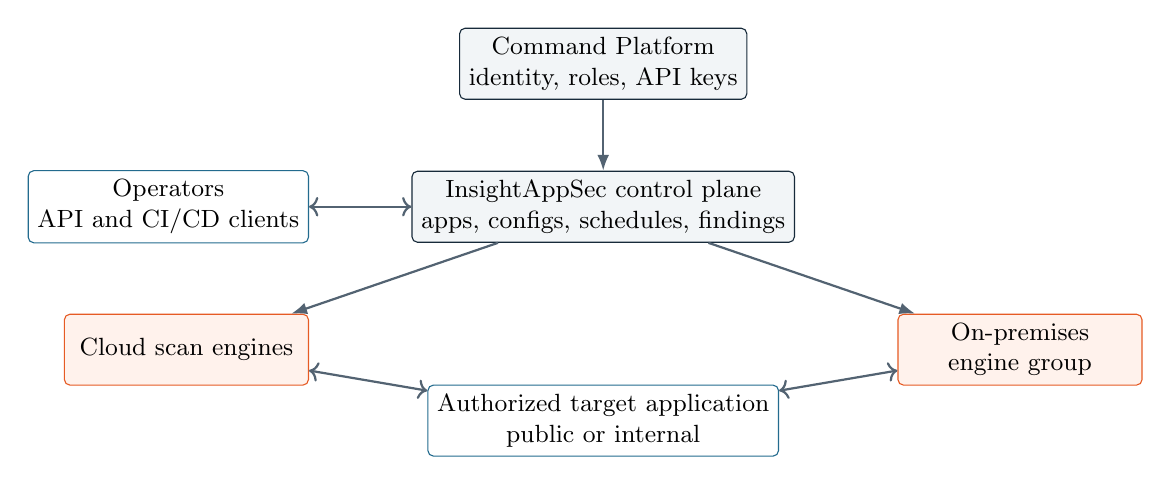
\begin{tikzpicture}[
  node distance=9mm and 13mm,
  box/.style={draw=R7Navy,rounded corners=2pt,fill=R7Light,minimum height=9mm,minimum width=31mm,align=center,font=\small},
  exec/.style={box,draw=R7Orange,fill=R7PaleOrange},
  ext/.style={box,draw=R7Blue,fill=white},
  arr/.style={-{Latex[length=2mm]},thick,draw=R7Slate}
]
\node[box] (cp) {Command Platform\\identity, roles, API keys};
\node[box,below=of cp] (ias) {InsightAppSec control plane\\apps, configs, schedules, findings};
\node[ext,left=of ias] (clients) {Operators\\API and CI/CD clients};
\node[exec,below left=of ias] (cloud) {Cloud scan engines};
\node[exec,below right=of ias] (onprem) {On-premises\\engine group};
\node[ext,below=18mm of ias] (target) {Authorized target application\\public or internal};
\draw[arr] (cp) -- (ias);
\draw[arr,<->] (clients) -- (ias);
\draw[arr] (ias) -- (cloud);
\draw[arr] (ias) -- (onprem);
\draw[arr,<->] (cloud) -- (target);
\draw[arr,<->] (onprem) -- (target);
\end{tikzpicture}
\end{center}

The on-premises engine polls the platform for tasks and updates and sends results to the platform; it must reach documented regional platform and engine endpoints.\src{S05} The platform chooses the first available member of a selected engine group. No official documentation reviewed establishes customer control over a more specific load-balancing algorithm.

\section{Scan lifecycle}
The UI documents the conceptual states Pending, Running, Scanned, Processed, Complete, Paused, Blacked Out, and Failed.\src{S02} The API exposes a more granular state enumeration, including queued, provisioning, awaiting-authentication, transition states, and canceled-as-failure semantics.\src{S38}

\begin{center}
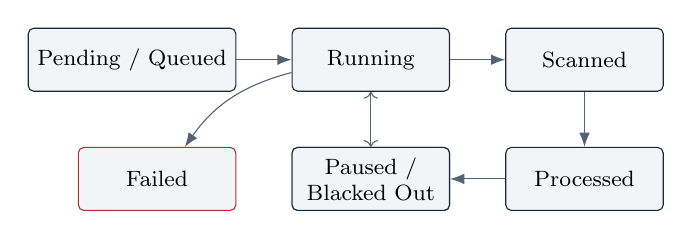
\begin{tikzpicture}[
  node distance=7mm and 7mm,
  state/.style={draw=R7Navy,rounded corners=2pt,fill=R7Light,minimum height=8mm,minimum width=20mm,align=center,font=\footnotesize},
  arr/.style={-{Latex[length=1.8mm]},draw=R7Slate}
]
\node[state] (p) {Pending / Queued};
\node[state,right=of p] (r) {Running};
\node[state,right=of r] (s) {Scanned};
\node[state,below=of s] (pr) {Processed};
\node[state,left=of pr] (c) {Complete};
\node[state,below=of r] (pa) {Paused /\\Blacked Out};
\node[state,left=of pa,draw=R7Red] (f) {Failed};
\draw[arr] (p) -- (r);
\draw[arr] (r) -- (s);
\draw[arr] (s) -- (pr);
\draw[arr] (pr) -- (c);
\draw[arr,<->] (r) -- (pa);
\draw[arr] (r) to[bend right=20] (f);
\end{tikzpicture}
\end{center}

\section{Regionality and reachability}
The API base URL is regional: \code{https://<region>.api.insight.rapid7.com/ias/v1}. Current documented region codes are \code{us}, \code{us2}, \code{us3}, \code{eu}, \code{ca}, \code{au}, \code{ap}, \code{me1}, and \code{aps2}. Determine the assigned data region on Platform Home and use that exact region.\src{S44}

Cloud engine IP allowlists are also regional and can change. Rapid7 publishes the current table and directs customers to identify the region from the product URL or Platform Home.\src{S04} This guide deliberately does not duplicate those IPs; use the current official table during every network change.

\chapter{Planning and Prerequisites}
\chapterlead{Turn a scan request into an authorized, reachable, measurable, and recoverable service operation.}

\section{Decisions to make before configuration}
\begin{enumerate}
  \item \textbf{Objective:} baseline, release gate, targeted validation, authenticated coverage, API/GraphQL/LLM assessment, or incident-driven verification.
  \item \textbf{Environment:} representative test/staging is preferred; production requires an explicit risk decision and operational controls.
  \item \textbf{Ownership:} application owner, technical contact, AppSec owner, remediator, change approver, and incident contact.
  \item \textbf{Engine:} cloud for public reachability or an on-premises engine group for internal reachability.\src{S05}
  \item \textbf{Identity:} dedicated test accounts, role coverage, MFA/bootstrap plan, secret custodian, and reset/revocation path.
  \item \textbf{Scope:} allowed domains, ports, seed URLs, inclusion/exclusion rules, APIs/schemas, and prohibited workflows.
  \item \textbf{Safety envelope:} time window, traffic limit, health signals, abort authority, monitoring, backup, and recovery test.
  \item \textbf{Evidence:} scan ID, config ID/version, crawl map, logs, report, vulnerability export, approvals, and change record.
\end{enumerate}

\section{Platform and engine prerequisites}
The user must have the product permissions and app access needed for the intended action. Product administration does not automatically mean visibility into every app's data; app access remains relevant.\src{S08}\src{S09}

For an on-premises engine, Rapid7 documents a platform/product administrator prerequisite and recommends 8 GB RAM, 100 GB free disk after the operating system, four CPU cores, and one network interface. The documented 64-bit Windows support set is Windows 10/11 and Windows Server 2016/2019/2022, with .NET Framework 4.8, Internet Explorer 11 or later, and Chrome on the engine host for Selenium macros.\src{S05} Treat the current source as authoritative if its requirements change.

\begin{oprec}
Capacity-size with a representative pilot, because application behavior, session complexity, crawl breadth, schemas, and attack selection can dominate runtime. Keep engine groups homogeneous in reachability and policy; alert on disk, memory, service, and outbound-connectivity conditions.
\end{oprec}

\section{Production readiness checklist}
\begin{longtable}{@{}P{0.28in}P{2.25in}P{3.95in}@{}}
\toprule
 & \textbf{Control} & \textbf{Acceptance evidence}\\
\midrule
\endhead
$\square$ & Written authorization & Target domains, environment, test class, window, and named approver are recorded.\\
$\square$ & Ownership and contacts & App owner, operator, change manager, network owner, identity owner, and abort contact are reachable.\\
$\square$ & Target allowlist & Domains are enabled in \uipath{Targets}; scope does not rely on stripped path components.\src{S03}\\
$\square$ & Engine reachability & Target is reachable from the selected cloud engine region or every eligible on-premises engine.\\
$\square$ & Platform connectivity & Required regional engine endpoints are reachable without TLS interception or proxy breakage.\src{S05}\\
$\square$ & App state and data & Test data exists; destructive or externally consequential actions are excluded or safely mocked.\\
$\square$ & Authentication & Test account is active, least privileged for the objective, and successfully verified; logout detection is configured.\src{S18}\\
$\square$ & Scope review & Seed URLs, restrictions, path rules, schema endpoints, file inputs, and redirects have peer review.\\
$\square$ & Load envelope & Template, threads, delays, and timeouts were proven in a controlled pilot; health monitors and abort thresholds exist.\\
$\square$ & Scheduling & Maintenance window, timezone, recurrence, blackout overlap, and maximum-pause behavior are understood.\src{S24}\\
$\square$ & Recovery & Backup/restore or rollback is viable; test account and data cleanup steps are assigned.\\
$\square$ & Notifications & Scan failure, bootstrap authentication, and on-premises engine offline notices reach staffed responders.\src{S11}\\
$\square$ & Evidence & Change ticket links config ID, engine group, app ID, operator, approval, monitoring dashboard, and log destination.\\
$\square$ & Stop authority & A named person can pause, stop-and-save, or cancel and understands the result implications.\src{S25}\src{S38}\\
$\square$ & Post-scan plan & Triage owner, response target, exception authority, retest plan, and evidence retention are defined.\\
\bottomrule
\end{longtable}

\chapter{Initial Configuration and Administration}
\chapterlead{Establish identity, least privilege, auditability, notifications, engines, and secrets before delegating scan work.}

\section{Users, groups, roles, and app access}
Rapid7 documents built-in Command Platform/product task roles including Admin, View and Change, View Only, App Owner, Scan Manager, and Remediator. Product feature access is expressed through Application Security permission groups (for example, Apps, Scans, and Attack Templates), while app access controls which app data a user or group can act on.\src{S08}\src{S45}

\begin{tabularx}{\textwidth}{@{}P{1.25in}P{2.15in}Y@{}}
\toprule
\textbf{Persona} & \textbf{Starting role} & \textbf{Access design}\\
\midrule
Platform administrator & Admin & Limit membership; administration alone should not be used as a substitute for app assignment.\\
App owner & App Owner & Assign only owned apps; can coordinate configuration and risk decisions within the documented permission set.\\
Scan operator & Scan Manager & Grant only apps and scan/configuration features required to build and operate scans.\\
Remediator & Remediator & Grant app visibility and finding workflow actions needed to review, comment, and validate.\\
Read-only stakeholder & View Only & Assign scoped app access for dashboards, reports, and evidence review.\\
Automation identity & Minimum custom or task role & Prefer a dedicated user key whose owner has only required product/app permissions.\\
\bottomrule
\end{tabularx}

\begin{procedure}{Provision an operator with least privilege}
\field{Purpose}Give a person or group only the functions and app data required for an assigned duty.
\field{When}Before onboarding, scanning, triage, reporting, or integration work.
\field{Prerequisites}Platform administrator access; approved persona and app list.
\field{Required role}Platform administrator for role/user administration; App Owner or administrator for app assignment as permitted.
\field{Security considerations}Avoid using Admin for routine scanning. Separate administration from automation. Review group nesting and inherited app access.
\field{Steps}
\begin{enumerate}
  \item In Command Platform administration, add or identify the user/group and assign the narrowest built-in or custom role that covers the task.\src{S45}
  \item In Application Security, open the app and use the documented user-access management view to assign the person/group to that app.\src{S10}
  \item Have the recipient sign in and perform a read-only check, then the smallest intended action in a non-production app.
  \item Record role, group, app list, approver, and review date.
\end{enumerate}
\field{Expected result}The user can perform intended actions only for assigned apps and cannot access administrative or unrelated app data.
\field{Validation}Test both a permitted and a deliberately unassigned app; inspect the effective access and audit record.
\field{Troubleshooting}If product features are visible but data is absent, check app access. If app data is visible but actions are disabled, check feature permissions.\src{S09}
\field{Rollback}Remove app assignment, then role/group membership; confirm access removal.
\field{Sources}\src{S08}\src{S09}\src{S10}\src{S45}
\end{procedure}

\section{Audit logging}
Application Security audit logging records manual and automated activity involving apps, targets, scan configurations, and files. An administrator is required to enable and view audit logging.\src{S07} Enable it before delegated administration or API adoption so an investigation has actor and time context.

\begin{procedure}{Enable and verify Application Security audit logging}
\field{Purpose}Capture attributable configuration and resource changes.
\field{When}During initial setup and after any tenant migration or navigation change.
\field{Prerequisites}Administrator access and an approved retention/evidence process.
\field{Required role}Administrator.
\field{Security considerations}Audit data can contain sensitive operational metadata; restrict export and retention locations.
\field{Steps}Follow the current \uipath{Settings > Audit Logging} workflow documented by Rapid7 to enable logging. Create a harmless test change (for example, update an approved description), then open the audit view and locate the actor, time, and action.\src{S07}
\field{Expected result}Both manual and automated test activity is represented in the audit view.
\field{Validation}Export or capture the agreed evidence and reconcile it to the change ticket.
\field{Troubleshooting}Confirm administrator permission, time filter, organization context, and that a documented event type was tested.
\field{Rollback}Revert the test change. Do not disable logging merely to remove test evidence.
\field{Sources}\src{S07}
\end{procedure}

\section{Notifications and webhooks}
Email preferences cover failed scans, scans awaiting bootstrap authentication, and on-premises engines going offline. Preferences are per user; recipients depend on event and app access.\src{S11} Webhooks support universal HTTP endpoints, Slack, and Microsoft Teams. Universal webhooks can use an HMAC algorithm and secret; integrations select triggers, filters, and apps.\src{S12}

\begin{procedure}{Configure and validate a universal webhook}
\field{Purpose}Send a documented scan event to an approved receiver.
\field{When}After receiver ownership, authentication, and data handling are approved.
\field{Prerequisites}HTTPS receiver, secret-storage plan, expected payload contract, and app/event selection.
\field{Required role}Permission to manage Application Security notifications/integrations.
\field{Security considerations}Use TLS, restrict endpoint access, validate HMAC when configured, prevent secret logging, and make receivers replay-tolerant.
\field{Steps}
\begin{enumerate}
  \item Go to \uipath{Settings > Notifications > Webhook Notifications > Create and Manage Webhooks}.\src{S12}
  \item Create a Universal webhook, enter the HTTPS endpoint, and configure the documented HMAC algorithm and secret if the receiver supports verification.
  \item Create an integration that selects the webhook, event trigger, filters, and apps.
  \item Run a controlled scan to completion. Capture the request metadata and confirm expected fields such as app ID/name, scan/config information, status, vulnerability count, timestamps, and deep link.
\end{enumerate}
\field{Expected result}Exactly the expected event is accepted and correlated to the scan.
\field{Validation}Verify signature, timestamp/event uniqueness in the receiver, HTTP success, and no secret exposure.
\field{Troubleshooting}Check app filter, trigger, receiver TLS, egress control, signature canonicalization, and receiver response logs.
\field{Rollback}Disable the integration first, then rotate/remove the secret and delete the webhook when no integrations depend on it.
\field{Sources}\src{S12}
\end{procedure}

\section{API keys}
User keys inherit the owner's current permissions and can be created by any user for their own account. Organization keys are platform-administrator-controlled ``super keys'' spanning products. Keys are displayed once; a lost key cannot be retrieved and must be replaced.\src{S39}\src{S46}

\begin{oprec}
Use a dedicated, least-privileged automation user and user key for routine InsightAppSec automation. Store the key in the CI or secrets platform, inject it at runtime, suppress shell tracing, never place it in source control, and rotate through an overlap-and-verify process. An organization key is broader than most scan automations need.
\end{oprec}

\section{On-premises engine setup}
\begin{procedure}{Install and pair an on-premises scan engine}
\field{Purpose}Provide execution capacity for internal targets that cloud engines cannot reach.
\field{When}After the host, region, outbound network path, and target path pass design review.
\field{Prerequisites}Current supported Windows host; documented CPU/RAM/disk/software; platform/product administrator; regional endpoint allowlisting; optional proxy details.\src{S05}
\field{Required role}Platform and product administrator as documented.
\field{Security considerations}Harden the dedicated host, limit interactive access, protect the setup key, avoid TLS interception, control target routes, and monitor the service and host.
\field{Steps}
\begin{enumerate}
  \item In \uipath{Settings > Manage Engines}, download the current installer and generate the setup API key.\src{S05}
  \item Run the installer on the prepared host. Let it validate requirements/connectivity; configure the approved proxy if required.
  \item Supply the setup key, name the engine, and save the pairing.
  \item Add it to an engine group whose members have equivalent target reachability. Leave automatic upgrade enabled unless an approved change process requires otherwise.\src{S05}\src{S06}
  \item Confirm the engine reports \emph{Online}. In a non-production app, set \uipath{Apps > Scan Config > Engine Groups} to the group and run a minimal scan.
\end{enumerate}
\field{Expected result}The engine is paired, online, selectable through its group, and able to reach the intended target.
\field{Validation}Record engine/group IDs and version, platform events, test scan ID, target response, host resource baseline, and update policy.
\field{Troubleshooting}Check regional hostnames, DNS, proxy authentication, outbound HTTPS, system clock, host requirements, service state, and target route/firewall.
\field{Rollback}Remove the engine from scheduling, finish or stop work safely, unpair/uninstall using the official procedure, and revoke exposed setup material.
\field{Sources}\src{S05}\src{S06}
\end{procedure}

\begin{safetybox}[Engine key regeneration is disruptive]
Rapid7 says to regenerate an engine API key only when compromised. A busy engine becomes unavailable and loses in-progress activities. The replacement must be updated in both \code{restclient-platform.cfg} and \code{upgraderestclient-platform.cfg}.\src{S14}
\end{safetybox}

\chapter{Application Onboarding}
\chapterlead{Create an application boundary only after its ownership, target authorization, scope, identity, and evidence model are clear.}

\section{Onboarding sequence}
\begin{enumerate}
  \item Approve the application and environment; complete the worksheet in \cref{sec:onboarding-worksheet}.
  \item Add the domain to \uipath{Targets}. Only the domain is retained; paths belong in app/scan scope.\src{S03}
  \item Create the app and associate target URLs and users.\src{S13}
  \item Create a named scan configuration that expresses one objective and one environment.\src{S15}
  \item Select cloud or on-premises engine group; verify source reachability.
  \item Configure scope, authentication, attack template, performance, schedules, and blackout protection.
  \item Run an unauthenticated/minimal pilot, validate the crawl map and logs, then introduce authentication and active testing.
  \item Baseline findings, ownership, exceptions, reporting, and retest workflow.
\end{enumerate}

\begin{procedure}{Add a target and create an app}
\field{Purpose}Create the governed product boundary for an authorized application.
\field{When}After onboarding approval and before any scan configuration.
\field{Prerequisites}Approved app name/description, target domains, URLs, owners, users/groups, environment, and engine decision.
\field{Required role}Target/app creation permissions plus appropriate app administration access.
\field{Security considerations}Confirm domain ownership/authorization; do not treat a parent-domain authorization as approval for every subdomain. Avoid production secrets in descriptions.
\field{Steps}
\begin{enumerate}
  \item Open \uipath{Targets > Add Targets}; enter one domain per line and select \uipath{Add Targets}. Confirm new targets are enabled.\src{S03}
  \item Open \uipath{Apps > Add App}. Complete \uipath{Details}, \uipath{Target URLs}, and \uipath{Users} using the approved worksheet.\src{S13}
  \item Confirm users/groups have the intended app access and that no unrelated principal was inherited.
  \item Record app ID, targets, owners, and environment tag in the service inventory.
\end{enumerate}
\field{Expected result}The app exists with only approved targets and users and is ready for a scan configuration.
\field{Validation}Open the app, verify target URLs and users, and test access with one allowed and one unassigned account.
\field{Troubleshooting}If a URL cannot be selected, verify its domain is enabled in Targets. If the domain was previously used, archive/disable rather than delete.\src{S03}
\field{Rollback}Remove unintended user access. Delete the app only after confirming it holds no required scans/findings; otherwise correct or decommission through the approved retention process.
\field{Sources}\src{S03}\src{S10}\src{S13}
\end{procedure}

\section{Onboarding worksheet}\label{sec:onboarding-worksheet}
\begin{longtable}{@{}P{1.8in}P{4.8in}@{}}
\toprule
\textbf{Field} & \textbf{Required answer / evidence}\\
\midrule
\endhead
Business/app name & Stable portfolio name, purpose, service tier, data classification, and inventory/CMDB identifier.\\
Environment & Development, test, staging, or production; deployment cadence and representative-data caveats.\\
Owners & Business owner, app owner, technical contact, AppSec contact, remediator, change/incident contacts.\\
Authorization & Approved domains/subdomains/IPs, environment, active/passive test class, dates, approver, and exclusions.\\
Target URLs & Exact seed URLs, protocols, ports, base paths, redirects, alternate hosts, and expected canonical domain.\\
Network & Public/internal, chosen region, cloud IP allowlist or on-prem group, DNS/proxy/WAF/CDN behavior, mutual TLS.\\
Scope & Included/excluded paths, maximum links, logout/delete/purchase/email/payment workflows, upload/download limits.\\
Authentication & Method, login URL, test identities/roles, MFA/bootstrap plan, session/logout indicators, rotation owner.\\
API/schema inputs & Swagger/OpenAPI/WSDL/GraphQL files/URLs, base endpoints, required headers, LLM chatbot endpoints/tags.\\
Scan objective & Baseline, release gate, scheduled surveillance, authenticated coverage, API coverage, or validation.\\
Safety envelope & Window, timezone, concurrency/delay starting point, health SLOs, abort signals, stop authority, rollback.\\
Evidence & Required reports/exports, scan logs, crawl map, retention, ticket linkage, dashboard stakeholders.\\
Workflow & Severity/status owner, issue tracker, exception approver/expiry, remediation target, retest trigger.\\
Acceptance criteria & Successful authentication, intended routes reached, excluded routes absent, request failure acceptable, no target-health regression.\\
\bottomrule
\end{longtable}

\begin{oprec}
Name apps and scan configurations with stable, searchable semantics, for example \code{payments-api / staging / authenticated-baseline}. Put volatile release identifiers in tags, tickets, or execution evidence rather than creating a new app for each build.
\end{oprec}

\chapter{Scan Configuration}
\chapterlead{Build configurations from the outside in: engine and target, then scope and crawl, then authentication, then attack selection and performance.}

\section{Create the configuration shell}
Open the app, select \uipath{Scan Configs > Create New Scan Config}, and give the configuration a unique objective-oriented name. The configuration is reusable; edits therefore affect later runs and should be change-controlled.\src{S15}

\section{Scope and crawl}
The Scan Scope area controls seed URLs, crawling restrictions, maximum links, and supplied interface descriptions such as WSDL and Swagger/OpenAPI.\src{S16} App target URLs produce default domain restrictions; a scan configuration can override them.\src{S17}

\begin{procedure}{Configure and prove scan scope}
\field{Purpose}Reach intended interfaces without crossing approved boundaries or triggering prohibited actions.
\field{When}For every new configuration and after material routing, UI, or API changes.
\field{Prerequisites}Approved seed URLs, domain/port/path map, exclusion list, schemas/traffic files, and target allowlist.
\field{Required role}Scan configuration edit permission and app access.
\field{Security considerations}Treat logout, delete, purchase, messaging, file upload, administrative, and external-redirect routes as high risk. Inspect supplied files for credentials.
\field{Steps}
\begin{enumerate}
  \item Open the app and scan configuration, then \uipath{Scan Scope}. Confirm seed URLs and generated target restrictions.\src{S16}\src{S17}
  \item Add the narrowest required inclusion and exclusion patterns. Configure maximum links according to the objective and proven capacity.
  \item Add approved Swagger/OpenAPI or WSDL inputs and use restriction options when the objective is API-only. Do not assume app URLs can be fully configured through the REST API; the public API specification says they currently cannot.\src{S38}\src{S40}
  \item Save and run a passive or otherwise constrained pilot. Export the crawl map from \uipath{Scans > [scan] > Crawl Map > Export JSON}.\src{S27}
  \item Compare discovered hosts/paths with the worksheet. Amend scope and repeat until inclusions and exclusions are evidenced.
\end{enumerate}
\field{Expected result}The crawl reaches approved paths and omits prohibited hosts and actions.
\field{Validation}Crawl map, request/log samples, target telemetry, and authentication state all match the acceptance criteria.
\field{Troubleshooting}Use supplied traffic for stateful sequences, inspect duplicate content, check literal versus wildcard matching, validate redirects and JavaScript routes, and review advanced crawl options only with evidence.\src{S26}
\field{Rollback}Restore the last approved configuration copy or reverse the individual scope change; cancel any run that crosses authorization boundaries.
\field{Sources}\src{S16}\src{S17}\src{S26}\src{S27}\src{S38}
\end{procedure}

\section{Authentication methods}
Rapid7 groups authentication into site, browser/HTTP, certificate, and server-level mechanisms.\src{S18} The choice should follow the application's actual authentication boundary and the engine type.

\begin{landscape}
\begin{longtable}{@{}P{1.10in}P{1.25in}P{1.95in}P{1.95in}P{2.05in}@{}}
\toprule
\textbf{Method} & \textbf{Use when} & \textbf{Prerequisites / configuration} & \textbf{Principal risks} & \textbf{Validation and common failures}\\
\midrule
\endhead
Automated Login & Standard or modern form login that the engine can identify & \uipath{Authentication > Site Authentication > Automated Login}; username/password; optional AppSec Chrome Extension verification; authenticated-only canary and logged-out redirect regex. & Account lockout, unintended privileged state, credentials retained in config (encrypted after save). & Verify before save; credentials must be re-entered to re-verify a saved config. Confirm canary and relogin in scan events.\src{S18}\\
Recorded macro (\code{.rec}) & Multi-step browser login or workflow & Rapid7 AppSec Chrome Extension; record/replay; on-premises host needs Chrome. & Macro captures secrets or brittle selectors; workflow causes state changes. & Replay interactively, then confirm Logged In and authenticated-only routes. Update after UI/identity changes.\src{S18}\\
Selenium IDE (\code{.side}) & Existing Selenium IDE login/workflow is maintainable & Supported Selenium side file and compatible engine/browser. & Timing and selector fragility; embedded secrets. & Run the file outside and inside the scan path; inspect event logs.\src{S18}\\
Traffic replay & Stateful API or browser requests are already captured & Supported \code{.trec}, Burp XML, Paros TXT, WebScarab conversation log, HAR, or Fiddler SAZ file. & Tokens/PII in capture; stale nonces; replayed mutations. & Sanitize, replay in test, verify response sequence and resulting crawl.\src{S18}\\
Session hijacking & A controlled session cookie is the intended bootstrap & Valid session cookie and session lifetime sufficient for the run. & High-value bearer material, expiry, user/session collision. & Confirm authenticated canary; ensure logout detection and rotation/revocation plan.\src{S18}\\
Bootstrap MFA & Interactive authentication is unavoidable & Latest Chrome extension; on-premises engine at least 7.2.049 where used; responder staffed for \emph{Awaiting Authentication}. & Human delay, 24-hour scan pause limit, social/approval fatigue. & Select \uipath{Authenticate Scan}; verify \emph{Logged In} in events and protected content.\src{S18}\\
Basic / NTLM / Kerberos & HTTP or integrated server authentication protects the site & Correct realm/domain identity and engine connectivity. Current August 2026 release notes document NTLM, Kerberos, and Negotiate support for Chromium-based scanning of internal targets. & Service-account privilege, delegation, lockout, platform/browser compatibility. & Test challenge/response from the selected engine; inspect 401/redirect loops and events.\src{S18}\src{S48}\\
HMAC & Requests require a documented HMAC signature & Username/secret; MD5, SHA1, or SHA256; custom DLL option requires on-premises engine. & Secret/DLL custody, algorithm weakness, clock/canonicalization mismatch. & Compare a signed known-good request; check timestamps and header canonicalization.\src{S18}\\
Client certificate (PFX) & Mutual TLS gates the application & PFX and password; cloud or on-premises engine according to current config. & Private-key exposure and expiration; wrong chain/SNI. & Verify handshake and authenticated endpoint from selected engine; protect and rotate PFX.\src{S18}\\
OAuth 2.0 & Standard authorization-code, implicit, resource-owner-password, or client-credentials flow & Authorization/token endpoints, client, scope, redirect, and grant-specific fields. PKCE is documented as unsupported. & Broad scopes, refresh-token exposure, unsupported modern flow, consent prompts. & Validate token issuance/refresh and protected canary. Use a macro workaround only where documented and tested.\src{S18}\\
MSAL & Microsoft identity flow using certificate credentials & PFX key file/password, tenant ID, client ID, scope, refresh period of at least 10 minutes. & Certificate and tenant/app privilege; expiry and consent. & Confirm token refresh beyond first period and protected content access.\src{S18}\\
\bottomrule
\end{longtable}
\end{landscape}

\begin{safetybox}[Authentication data]
Use non-personal test identities and synthetic data. Captures, macros, cookies, PFX files, OAuth secrets, HMAC secrets, and scan configuration exports can all contain credentials or bearer material. Restrict access, retention, and logs; revoke or rotate them at the end of testing.
\end{safetybox}

\section{Attack templates and modules}
Default templates bundle common attacks and performance options; custom templates allow enable/disable choices, severity, maximum findings, attack location, false-positive regex, and attack-per-input behavior. Active attacks send payloads and can alter target behavior; passive attacks inspect observed traffic.\src{S02}\src{S19}\src{S20}

\begin{oprec}
Start from the narrowest default template that meets the objective, then create a named custom template only when the exception is durable and documented. Run ``All modules'' in pre-production unless a production risk acceptance explicitly authorizes it; Rapid7 itself warns that this template can significantly slow or disrupt customer-facing websites.\src{S19}
\end{oprec}

\section{Custom and advanced options}
Custom Options includes proxy, performance, headers, and advanced settings. Rapid7 documents a default URL retry behavior, 25 ms minimum delay, 200 ms as a suggested light-load delay, and a 60,000 ms connection timeout, but these are product defaults/suggestions rather than a guarantee of safety for a specific target.\src{S21}

Advanced Options exposes expert-level engine settings. For example, \code{TreatFailedReloginAsError} defaults to \code{1}, which causes a scan to stop when relogin fails; \code{AccountType} is documented as deprecated.\src{S22} Treat advanced-option names and effects as version-sensitive and preserve a tested rollback value.

\section{API, WSDL, GraphQL, and LLM surfaces}
\subsection{Swagger/OpenAPI and WSDL}
Add the approved schema/file in Scan Scope and set the documented restriction if the objective is limited to that interface. Verify base URLs, authentication headers, server variables, and examples against the deployment; a syntactically valid description can still point at the wrong environment.\src{S16}

\subsection{GraphQL}
In \uipath{Scan Scope > GraphQL}, upload a \code{.gql} (JSON) or \code{.graphqls} (SDL) file, or provide an introspection query URL. Configure GraphQL endpoint URL, verb, maximum requests, and host; at least the endpoint URL or host must be populated, then enable and save. The documented GraphQL template includes injection, OS commanding, SSRF, and file-inclusion tests.\src{S23}

\subsection{LLM scanning}
Rapid7 documents LLM scanning with macro or CSS-selector workflow inputs and Swagger/OpenAPI endpoints tagged \code{chatbot}. The CSS Page URL must follow the documented constraints. Rapid7 states that foundation LLMs used by the feature remain within its cloud boundary and that customer data is not used to train/fine-tune Rapid7 or third-party models.\src{S47}

\subsection{AI-enhanced attack validation}
AI-enhanced attack modules require View and Change Attack Templates permission and a cloud engine; on-premises engines are unsupported. As of the cutoff, the official page says the feature is unavailable in APS2 and ME regions and that CA may vary. AI-flagged false positives are excluded from results.\src{S49} August 2026 release notes describe AI validation expansion, including SQL injection and remote file inclusion using AWS Bedrock.\src{S48}

\begin{docgap}[AI availability and auditability]
The feature page and recent release notes evolve rapidly. Reconfirm region and module availability in the tenant. Because AI-excluded findings do not appear in results, organizations requiring independent comparison should run a controlled, approved comparison without the AI option; that comparison is an operational recommendation, not a documented Rapid7 requirement.
\end{docgap}

\section{Schedules and blackouts}
Schedules define date, time, and recurrence. Blackouts pause running scans, and a scan scheduled during a blackout queues until the blackout ends. A pause cannot exceed 24 hours; after the limit the scan stops and partial results are retained.\src{S24}\src{S25}

\begin{procedure}{Schedule a recurring scan with blackout protection}
\field{Purpose}Run an approved configuration predictably while preserving protected operational windows.
\field{When}After at least one successful, monitored manual execution.
\field{Prerequisites}Stable config, timezone, recurrence, maintenance window, blackout calendar, owner, and failure recipient.
\field{Required role}Schedule/scan management permission and app access.
\field{Security considerations}Avoid overlap with deployments, batch processing, backup, and identity maintenance; do not rely on blackout for pauses longer than 24 hours.
\field{Steps}Open the app/configuration scheduling view, create the schedule with explicit timezone/recurrence, then create blackouts for protected intervals. Enable relevant failure/offline/authentication email preferences.\src{S11}\src{S24}
\field{Expected result}The scan starts at the intended local time, or queues until blackout ends.
\field{Validation}Observe the first scheduled run and blackout interaction; reconcile timestamps and status events.
\field{Troubleshooting}Check timezone, disabled target/config, engine availability, overlapping blackout, and license/configuration status.
\field{Rollback}Disable/delete the schedule and confirm no queued scan remains; cancel or stop an unintended run according to evidence needs.
\field{Sources}\src{S11}\src{S24}\src{S25}
\end{procedure}

\chapter{Run and Monitor Scans}
\chapterlead{Execute scans as observable operations with a known owner, explicit abort authority, and evidence sufficient to explain coverage and failure.}

\section{Manual execution}
From the app, select \uipath{Scan Now}, choose a scan configuration, and start the run. The Scan Overview presents vulnerabilities and scan logs. Running scans can be paused/resumed, stopped with results saved or discarded through the documented UI choices, or managed through API actions.\src{S25}

\begin{procedure}{Start and monitor an approved scan}
\field{Purpose}Execute a configuration while continuously validating target health, authentication, coverage, and engine state.
\field{When}At the approved change window or release-gate event.
\field{Prerequisites}Completed readiness checklist; approved config; reachable target/engine; staffed target, scan, and incident contacts.
\field{Required role}Scan execution permission and app access.
\field{Security considerations}Confirm environment and seed URL immediately before start. Never copy a production credential into a staging configuration or vice versa. Keep abort actions available.
\field{Steps}
\begin{enumerate}
  \item Open the app and select \uipath{Scan Now}; select the approved configuration and start.\src{S25}
  \item Record app ID, scan configuration ID, scan ID, operator, engine group, start time, and change ticket.
  \item In \uipath{Scan Overview}, watch status, vulnerability count, Scan Logs, platform/engine events, authentication messages, request failures, and crawl progress.
  \item In parallel, watch target latency, error rate, saturation, security controls, external side effects, and test-account state.
  \item If the safety envelope is crossed, pause for a short diagnosis, stop and retain partial results when evidence is useful, or cancel when the operation must be abandoned. A pause beyond 24 hours becomes a stop with partial results retained.\src{S24}\src{S25}
  \item At completion, export/record the crawl map and reconcile observed coverage with the objective.
\end{enumerate}
\field{Expected result}The scan reaches Complete without crossing the safety envelope; intended authenticated routes and APIs appear in evidence.
\field{Validation}Check logs, authenticated canary, crawl map, target telemetry, completed timestamps, findings, and configuration identity.
\field{Troubleshooting}Use the status-code table in \cref{ch:troubleshooting}; investigate engine, network, target, scope, authentication, and resource conditions before rerun.
\field{Rollback}Stop/cancel the scan; disable schedule if applicable; recover target state/data; revoke temporary credentials; restore prior configuration; open an incident if impact occurred.
\field{Sources}\src{S24}\src{S25}\src{S26}\src{S27}\src{S37}
\end{procedure}

\section{Stop versus cancel}
Rapid7 distinguishes a long-running scan stop intended to gather results from canceling a scan. In the REST API both use \code{PUT /scans/\{id\}/action}: \code{STOP} enters the result-producing stop flow, while \code{CANCEL} forces a canceled failure state.\src{S38}\src{S41}

\begin{safetybox}[Choose the terminal action deliberately]
Use \emph{stop} when partial processing/evidence is valuable and the target is stable enough for a controlled finish. Use \emph{cancel} when the run must be abandoned. Record the reason, actor, time, target state, and resulting status. Do not describe a canceled scan as a completed assessment.
\end{safetybox}

\section{Logs and crawl validation}
The event stream should explain state transitions, engine activity, authentication/relogin, and failures. The crawl map provides a JSON representation of discovered topology and is exported as \code{<scan\_name>-crawl-map.json}.\src{S27} Compare it with the onboarding worksheet; a large link count is not equivalent to meaningful functional coverage.

\section{Failed scan status families}
Rapid7 documents platform conditions such as \code{BOOTSTRAP\_}\allowbreak\code{AUTHENTICATION\_}\allowbreak\code{FAILURE}, \code{ENGINE\_UNAVAILABLE}, \code{CANCELED}, \code{CONFIGURATION\_INVALID}, \code{LICENSE\_INVALID}, and \code{SYSTEM\_ERROR}; engine-level conditions include \code{BAD\_AUTH}, \code{DATABASE\_TOO\_LARGE}, initialization, disk/memory, network, and report-generation failures.\src{S37} Preserve the exact code and the \code{r7-correlation-id} when escalating API-related problems.\src{S38}

\section{Full, incremental, and validation scans}
Use a full/regular scan for comprehensive reassessment of the configured surface. Incremental scanning is a configuration option for change-oriented work. Validation focuses on selected existing findings; Rapid7 recommends it for remediation testing but notes it is not as comprehensive as a full scan and can still produce new findings.\src{S15}\src{S25}

\chapter{Vulnerability Analysis and Triage}
\chapterlead{Make triage reproducible: inspect evidence, establish reachability and impact, set a governed status, and preserve the rationale.}

\section{Finding evidence}
The vulnerability detail includes age, severity, request, response, and related evidence. Review the discovery in its application context, including the authenticated role, target path, input location, server behavior, and whether controls changed or normalized the request.\src{S29}

\section{Statuses and semantics}
\begin{tabularx}{\textwidth}{@{}P{1.25in}Y P{2.15in}@{}}
\toprule
\textbf{Status / marker} & \textbf{Documented meaning and persistence} & \textbf{Operator evidence}\\
\midrule
Unreviewed & Default workflow state requiring assessment. A rediscovered item previously marked Remediated returns to Unreviewed.\src{S28} & Initial evidence, owner, due date, triage notes.\\
New & A marker, not a manually assignable status.\src{S28} & First-seen scan and comparison baseline.\\
Verified & Finding has been reviewed and accepted as genuine. & Reproduction/evidence, impact, affected route/role.\\
Ignored & Finding is excluded from active work without asserting that it is false. & Reason, accountable owner, review/expiry date.\\
False Positive & Finding is judged not genuine; the status persists in subsequent scans.\src{S28} & Concrete request/response analysis and independent reviewer.\\
Duplicate & Finding maps to another tracked issue; status persists in subsequent scans.\src{S28} & Canonical finding/ticket and equivalence rationale.\\
Remediated & Finding is no longer observed under the relevant validation conditions. Rediscovery can return it to Unreviewed.\src{S28}\src{S32} & Validation result, scan ID/config, scope/auth equivalence, deployment.\\
\bottomrule
\end{tabularx}

\begin{procedure}{Triage a vulnerability}
\field{Purpose}Assign a defensible severity, status, owner, and next action from observed evidence.
\field{When}On new/unreviewed findings, rediscovery, or material application/control change.
\field{Prerequisites}App access; finding detail; scan/config/crawl context; application owner or technical contact.
\field{Required role}Remediator or a role with vulnerability view/change permission for the app.
\field{Security considerations}Requests/responses can contain tokens, PII, and exploit payloads. Use a restricted workspace; do not replay against production without authorization.
\field{Steps}
\begin{enumerate}
  \item Filter to the app/scan/severity/status of interest, then open the vulnerability.\src{S28}\src{S29}
  \item Inspect request, response, attack evidence, authenticated role, URL/input, age, and discovery history. Confirm the run had valid authentication and intended scope.
  \item Determine exploitability, data/action consequence, required preconditions, exposure, and relevant compensating controls. Do not reduce severity solely because a scan did not demonstrate maximum impact.
  \item Set the supported status and severity, add a concise comment with evidence and uncertainty, assign the remediation owner/ticket, and record the response/retest target.
  \item If False Positive, Duplicate, Ignored, or an exception is proposed, require the evidence and approval defined in policy.
\end{enumerate}
\field{Expected result}The finding has one accountable disposition, rationale, ticket, and next review/retest event.
\field{Validation}A second reviewer can reproduce the reasoning from product evidence and linked records; change history shows the action.
\field{Troubleshooting}If evidence is incomplete, inspect scan logs/crawl/authentication and use a controlled validation or Replay Attack rather than guessing.
\field{Rollback}Revert an incorrect status/severity and comment why; correct the external ticket and dashboard filters.
\field{Sources}\src{S28}\src{S29}\src{S31}\src{S32}
\end{procedure}

\section{Exceptions}
Exceptions can represent false positives, accepted risks, or compensating controls and hide covered vulnerabilities from the vulnerability page, dashboards, and scan details. A user needs the exception permission/role, and only one active exception can apply to a vulnerability.\src{S30}

\begin{oprec}
Require an accountable approver, category, rationale, compensating control, ticket, creation date, expiry/review date, and explicit scope for every exception. Review the hidden population separately so an exception never becomes silent deletion of risk.
\end{oprec}

\section{Triage quality checklist}
\begin{multicols}{2}
\begin{itemize}
  \item[$\square$] Scan/config/engine identified
  \item[$\square$] Authentication state verified
  \item[$\square$] Request/response protected
  \item[$\square$] Affected role and input recorded
  \item[$\square$] Reachability and preconditions assessed
  \item[$\square$] Business/data consequence described
  \item[$\square$] Compensating control verified
  \item[$\square$] Severity rationale written
  \item[$\square$] Status semantics match evidence
  \item[$\square$] Owner and ticket assigned
  \item[$\square$] Exception approval/expiry present
  \item[$\square$] Retest method and date defined
\end{itemize}
\end{multicols}


\chapter{Remediation and Retesting}
\chapterlead{Close findings only when a relevant deployment has been tested under equivalent reach, identity, and scope conditions.}

\section{Remediation workflow}
\begin{enumerate}
  \item Preserve the original evidence and scan/config identifiers.
  \item Translate the finding into a root-cause fix and add regression tests where possible.
  \item Deploy through the normal change process; record environment, build, and controls.
  \item Run a focused validation for rapid feedback, then a full scan when the assurance objective requires broad regression coverage.\src{S25}\src{S31}
  \item Reconcile the validation result and status transition; do not equate an authentication or coverage failure with remediation.
\end{enumerate}

\begin{procedure}{Validate remediation}
\field{Purpose}Determine whether a previously observed vulnerability is still found after an approved fix.
\field{When}After deployment to the testable environment and before closure.
\field{Prerequisites}Finding ID, fix/build evidence, reachable target, equivalent authentication/role, and a valid scan engine/config.
\field{Required role}Vulnerability validation permission and app access.
\field{Security considerations}Replay and validation send attack traffic. Verify environment and test data; avoid replaying captured bearer tokens outside their context.
\field{Steps}
\begin{enumerate}
  \item Open the finding and review the original request/response and discovery context.
  \item For an interactive check, use the Rapid7 AppSec Chrome plugin \emph{Replay Attack}; for engine-based confirmation, select the finding(s) and \emph{Validate Vulns}.\src{S31}
  \item Monitor authentication, engine events, and target health. Await result processing.
  \item Review the validation history and one of the documented outcomes: Found, Not found, Unconfirmed, or Not validated.\src{S32}
  \item If the assurance objective is broader than the specific finding, run a full scan after focused validation.
\end{enumerate}
\field{Expected result}A valid test produces a documented outcome tied to the finding and environment.
\field{Validation}Confirm the validation used the correct endpoint, role, deployment, and reachable path; inspect response rather than status alone.
\field{Troubleshooting}Unconfirmed/Not validated requires investigation of authentication, scope, reachability, target behavior, or engine conditions; it is not proof of remediation.
\field{Rollback}If the fix regresses function or increases risk, roll back the application change through its deployment process and reopen/reclassify the finding.
\field{Sources}\src{S25}\src{S31}\src{S32}
\end{procedure}

\section{Validation status transitions}
\begin{tabularx}{\textwidth}{@{}P{1.3in}P{1.55in}P{1.55in}P{1.55in}@{}}
\toprule
\textbf{Prior status} & \textbf{Found} & \textbf{Not found} & \textbf{Unconfirmed}\\
\midrule
Verified & Verified & Remediated & Verified\\
Unreviewed & Unreviewed & Remediated & Unreviewed\\
Remediated & Unreviewed & Remediated & Remediated\\
Ignored & Ignored & Remediated & Ignored\\
False Positive & False Positive & False Positive & False Positive\\
Duplicate & Duplicate & Duplicate & Duplicate\\
\bottomrule
\end{tabularx}
These transitions are the documented validation behavior; ``Not validated'' requires investigation rather than a closure inference.\src{S32}

\section{Closure evidence}
At minimum, retain the original and validation scan IDs, configuration ID/version, app/environment, authenticated role, fix/build/change ID, validation outcome, request/response comparison, status change actor/time, and whether a full regression scan followed.

\chapter{Dashboards, Reports, Exports, and Metrics}
\chapterlead{Use evidence views for different decisions: dashboards for portfolio signals, reports for communication, exports/API for analysis, and raw scan artifacts for technical verification.}

\section{Dashboards}
Dashboard filters include App ID, app tags, name, description, and date. Rapid7 recommends applying the global app filter where appropriate; dashboards can be refreshed and copied.\src{S34} Treat widgets as views of the current filtered dataset, not as immutable audit evidence.

\section{Reports}
Rapid7 documents executive, combined Application Security/Vulnerability Management, app executive, vulnerability summary, vulnerability remediation, and compliance-oriented reports, with PDF and HTML output. Compliance reports are advisory and do not affirm compliance.\src{S35}

\begin{safetybox}[Compliance caveat]
A report mapping findings to a framework is evidence input, not a certification or an attestation of control effectiveness. Record scope, scan date/configuration, authentication, exclusions, unresolved coverage gaps, exceptions, and the responsible compliance interpretation.
\end{safetybox}

\section{Exports}
Vulnerabilities can be exported from the global Vulnerabilities view, app vulnerability tab, or scan vulnerability tab to Jira, ServiceNow, or CSV.\src{S33} Crawl maps export to JSON.\src{S27} Broader data export options are documented separately.\src{S36}

\section{Metrics with decision value}
\begin{tabularx}{\textwidth}{@{}P{1.8in}Y P{1.75in}@{}}
\toprule
\textbf{Metric} & \textbf{Definition and use} & \textbf{Guardrail}\\
\midrule
Portfolio coverage & Apps with a successful qualifying scan in the policy window / in-scope apps. & Segment by environment and authenticated coverage.\\
Authenticated coverage & Qualifying scans with verified login and protected routes / scans expected to authenticate. & Do not infer from config presence alone.\\
Scan reliability & Complete qualifying scans / started scans, with failures by documented reason. & Separate canceled/change-window events.\\
Triage latency & Time from first observation to accountable status/owner. & Exclude neither false positives nor exceptions; track their review time.\\
Remediation latency & Time from verification/assignment to validated not-found/remediated state. & Segment by severity and app tier.\\
Rediscovery rate & Remediated findings later returned to Unreviewed / remediated findings. & Confirm same finding/coverage context.\\
Exception exposure & Active exception count/age by reason, severity, app, and expiry. & Include hidden vulnerabilities in governance reporting.\\
Crawl quality & Expected critical routes reached, prohibited routes absent, request-failure trend. & Link to worksheet and crawl map, not raw URL count.\\
\bottomrule
\end{tabularx}

\begin{oprec}
Define a ``qualifying scan'' locally (for example, correct environment, valid authentication, intended config, adequate reach, and Complete status) before computing trends. Rapid7 does not establish the policy thresholds, denominators, or service-level objectives in this table.
\end{oprec}

\chapter{Integrations and CI/CD}
\chapterlead{Automate only with documented integrations, protected credentials, explicit timeouts, version control, and a failure policy that distinguishes product risk from platform unavailability.}

\section{Common integration controls}
\begin{itemize}
  \item Store API keys/service credentials in the native secrets or managed-credential facility; never in workflow source or console output.
  \item Pin an approved action, plugin, extension, or image version when supported; review release changes before upgrades.
  \item Use a dedicated scan configuration ID and least-privileged user key.
  \item Decide separately how the pipeline handles vulnerability-gate failure, scan failure, timeout, cancellation, and unavailable platform/engine.
  \item Preserve workflow/build ID, commit, config/scan IDs, query, result, timing, and deep link as evidence.
\end{itemize}

\section{GitHub Actions}
The documented workflow is event $\rightarrow$ GitHub action $\rightarrow$ InsightAppSec scan $\rightarrow$ results $\rightarrow$ workflow continuation. It requires an API key stored as a secret and a scan configuration ID; a vulnerability query can fail a job as a gate.\src{S50}

The official documentation example pins \code{rapid7/insightappsec-scan-github-actions@v1.1.0}. The official Rapid7 repository has later tags, including \code{v1.5.1} visible at the cutoff.\src{S50}\src{S51} This is a material documentation/version discrepancy: do not infer compatibility from the tag name alone.

\begin{oprec}
Select an approved immutable tag after reviewing the official repository release/tag content and testing it in a non-production workflow. Record the chosen tag and upgrade owner; do not use a moving branch.
\end{oprec}

\section{GitLab CI/CD}
Rapid7 documents the container \code{rapid7/insightappsec-gitlab-scan:latest}, the script \code{python3 /insightappsec\_scan/actions.py}, an API key variable, scan configuration ID, region, and options for vulnerability query, wait behavior, log level, timeout, and failure on findings.\src{S52}

\begin{oprec}
The documentation's \code{:latest} tag is mutable. If the publisher provides a verifiable version or digest that works in the tenant, pin and periodically update it through change control; otherwise record the fetched digest in each build and test changes before promotion.
\end{oprec}

\section{Azure DevOps}
The documented extension uses a service connection containing the region and API token, then a task that selects app/configuration and options for waiting, polling, reports/artifacts, timeout/cancel behavior, and vulnerability-query gating.\src{S53} Treat build logs and generated reports as potentially sensitive because scan evidence and URLs can be visible to users with pipeline history access.

\section{Jenkins}
Rapid7's Jenkins integration supports freestyle and pipeline jobs and requires a Command Platform user with View and Change or Admin access; trial licenses cannot start scans through the API. It configures region, API key/managed credential, app, scan configuration, wait milestones, query, and pending/execution durations.\src{S54} Rapid7 warns that users with build-history access can see published results; scope Jenkins permissions accordingly.

\section{Jira}
Jira export creates issues and maps documented status/severity fields. Changes made in InsightAppSec are not automatically reflected in Jira and require an explicit re-export.\src{S55} Define which system owns status and how duplicates are reconciled.

\section{ServiceNow}
\subsection{ITSM}
The ITSM integration requires both relevant licenses and a ServiceNow user with documented roles; it uses an organization API key and supports two-way severity/status synchronization. The connection workflow is under \uipath{Settings > Integrations > Enable ServiceNow Integration} and includes a connection test.\src{S56}

\subsection{Application Vulnerability Response}
The AVR integration can fetch apps, scans, vulnerabilities, and attack details manually or periodically and supports two-way status handling.\src{S57} Establish reconciliation, deletion, exception, and conflict ownership before scheduled imports.

\section{Webhooks}
Use the universal/Slack/Teams workflow described in Chapter 4 for event notification; a webhook is not a replacement for polling the scan resource when an automation requires authoritative state. The official documentation does not establish exactly-once delivery or ordering guarantees. 

\section{Unsupported or not established}
The official Bamboo page is explicitly marked ``Not Supported''; do not design a new Bamboo integration from that page.\src{S58} For any CI/CD or ticketing system not covered above, use the public REST API only after confirming required operations and supportability. Product-native integrations with other systems are \notestablished

\chapter{REST API Operations}
\chapterlead{Use the official OpenAPI v1 contract as the endpoint/schema authority and the narrative guide for workflow context. Preserve status codes, Location headers, and correlation IDs.}

\section{Endpoint and authentication}
Use \code{https://<region>.api.insight.rapid7.com/ias/v1} with the assigned region code. Send the key in \code{X-Api-Key}; JSON requests use \code{Content-Type: application/json}, and clients should send an appropriate \code{Accept}.\src{S38}\src{S39}\src{S44}

\begin{lstlisting}[language=bash,caption={Safe shell setup for examples}]
export IAS_REGION='us'  # use the tenant's actual documented region
export IAS_BASE_URL="https://${IAS_REGION}.api.insight.rapid7.com/ias/v1"
# Inject INSIGHTAPPSEC_API_KEY from an approved secret store.
# Do not echo it and do not run these commands with shell tracing enabled.
\end{lstlisting}

User keys inherit the owner's permissions; organization keys are super keys controlled by platform administrators. Keys are shown once.\src{S39}\src{S46} Every example below assumes a least-privileged user key, existing authorization for the target, and IDs belonging to the correct tenant and environment.

\section{Connectivity test}
Command Platform documents a regional \code{/validate} authentication check. For product authorization and route validation, a safe \code{GET /apps?size=1} additionally proves the InsightAppSec v1 endpoint can list apps visible to the key.\src{S59}\src{S38}

\begin{lstlisting}[language=bash]
curl --fail-with-body --silent --show-error \
  -H "X-Api-Key: ${INSIGHTAPPSEC_API_KEY}" \
  -H 'Accept: application/json' \
  "${IAS_BASE_URL}/apps?size=1"
\end{lstlisting}
Expected: HTTP 200 and a paged JSON response. HTTP 401 indicates missing/invalid authentication; 403 indicates insufficient authorization; verify region before replacing the key.

\section{Pagination, filtering, errors, and safety semantics}
Collection endpoints use zero-based \code{index} (default 0), \code{size} (default 50; documented range 1--1000), \code{sort}, and, where returned, \code{page-token}. The token mechanism supports retrieval beyond the 10,000-result offset boundary; use the returned token unchanged for the next page.\src{S38}

The search endpoint accepts a type and case-sensitive query DSL. Filter properties/operators are resource-specific and must come from the current specification; do not interpolate untrusted strings.\src{S38}

Client errors are 4xx and server errors 5xx. Error bodies commonly include \code{status} and \code{message}; validation responses can contain \code{errors}. Preserve the response \code{r7-correlation-id} for support. Creation normally returns HTTP 201 with an absolute resource URL in \code{Location}.\src{S38}

\begin{docgap}[Rate limits and idempotency]
Numeric API rate limits and retry headers are \notestablished Formal idempotency guarantees or idempotency-key support are also \notestablished Treat POST creation/start calls as non-idempotent, retain the 201 \code{Location}, and reconcile existing resources before retrying after an ambiguous network outcome.
\end{docgap}

\begin{oprec}
For 429 or transient 5xx responses, use bounded exponential backoff with jitter only when the operation is safe to retry. For POST requests, first query for the intended resource or reconcile the captured Location/scan ID. Stop automatic retries on authentication, authorization, validation, and configuration errors.
\end{oprec}

\section{List applications}
\begin{lstlisting}[language=bash]
curl --fail-with-body --silent --show-error \
  -H "X-Api-Key: ${INSIGHTAPPSEC_API_KEY}" \
  -H 'Accept: application/json' \
  "${IAS_BASE_URL}/apps?size=50&index=0"
\end{lstlisting}
Expected: HTTP 200. Follow response metadata/page token until exhausted; record app IDs, not only names.

\section{Create a target and app}
\begin{lstlisting}[language=bash]
curl --fail-with-body --silent --show-error \
  -D target.headers -o target.json \
  -X POST "${IAS_BASE_URL}/targets" \
  -H "X-Api-Key: ${INSIGHTAPPSEC_API_KEY}" \
  -H 'Accept: application/json' \
  -H 'Content-Type: application/json' \
  --data '{"domain":"staging.example.test","enabled":true}'

curl --fail-with-body --silent --show-error \
  -D app.headers -o app.json \
  -X POST "${IAS_BASE_URL}/apps" \
  -H "X-Api-Key: ${INSIGHTAPPSEC_API_KEY}" \
  -H 'Accept: application/json' \
  -H 'Content-Type: application/json' \
  --data '{
    "name":"payments-api / staging",
    "description":"Authorized staging DAST boundary"
  }'
\end{lstlisting}
Expected: HTTP 201 and a \code{Location} header for each created resource. IDs sent in POST bodies are ignored by the API. App target URLs cannot currently be configured through the public API; add the domain as a target and configure scan options according to the documented workflow.\src{S38}\src{S40}

\section{Create a scan configuration}
First list attack templates and identify the approved template ID.
\begin{lstlisting}[language=bash]
curl --fail-with-body --silent --show-error \
  -H "X-Api-Key: ${INSIGHTAPPSEC_API_KEY}" \
  -H 'Accept: application/json' \
  "${IAS_BASE_URL}/attack-templates?size=100"

curl --fail-with-body --silent --show-error \
  -D scan-config.headers -o scan-config.json \
  -X POST "${IAS_BASE_URL}/scan-configs" \
  -H "X-Api-Key: ${INSIGHTAPPSEC_API_KEY}" \
  -H 'Accept: application/json' \
  -H 'Content-Type: application/json' \
  --data "{
    \"name\":\"payments-api / staging / baseline\",
    \"app\":{\"id\":\"${APP_ID}\"},
    \"attack_template\":{\"id\":\"${ATTACK_TEMPLATE_ID}\"}
  }"
\end{lstlisting}
Expected: HTTP 201 and \code{Location}. Then use \code{PUT /scan-configs/\{id\}/options} only with a complete, validated options document; \code{PATCH} is available for supported partial updates. Retrieve the current options first and preserve a rollback copy.\src{S38}\src{S40}

\section{Start and monitor a scan}
\begin{lstlisting}[language=bash]
curl --fail-with-body --silent --show-error \
  -D scan.headers -o scan.json \
  -X POST "${IAS_BASE_URL}/scans" \
  -H "X-Api-Key: ${INSIGHTAPPSEC_API_KEY}" \
  -H 'Accept: application/json' \
  -H 'Content-Type: application/json' \
  --data "{\"scan_config\":{\"id\":\"${SCAN_CONFIG_ID}\"}}"

# Extract SCAN_ID from the absolute Location header, then poll:
curl --fail-with-body --silent --show-error \
  -H "X-Api-Key: ${INSIGHTAPPSEC_API_KEY}" \
  -H 'Accept: application/json' \
  "${IAS_BASE_URL}/scans/${SCAN_ID}"
\end{lstlisting}
Expected start response: HTTP 201 plus \code{Location}. Poll at a controlled interval until a terminal status; documented states include Pending/Queued/Provisioning, Running, Scanned/Processed/Complete, Paused/Blacked Out/Awaiting Authentication, transitions, and Failed.\src{S38}\src{S41}

\section{Stop or cancel a scan}
\begin{lstlisting}[language=bash]
# Controlled stop: retains the result-producing stop workflow.
curl --fail-with-body --silent --show-error \
  -X PUT "${IAS_BASE_URL}/scans/${SCAN_ID}/action" \
  -H "X-Api-Key: ${INSIGHTAPPSEC_API_KEY}" \
  -H 'Accept: application/json' \
  -H 'Content-Type: application/json' \
  --data '{"action":"STOP"}'

# Emergency abandon: use CANCEL deliberately.
curl --fail-with-body --silent --show-error \
  -X PUT "${IAS_BASE_URL}/scans/${SCAN_ID}/action" \
  -H "X-Api-Key: ${INSIGHTAPPSEC_API_KEY}" \
  -H 'Accept: application/json' \
  -H 'Content-Type: application/json' \
  --data '{"action":"CANCEL"}'
\end{lstlisting}
Expected: HTTP 200 for an accepted action, followed by a transition such as Stopping or Canceling. Re-read the scan until terminal and record the final status/failure reason. Supported actions also include Pause, Resume, and Authenticate.\src{S38}

\section{Retrieve vulnerabilities}
\begin{lstlisting}[language=bash]
# List visible vulnerabilities.
curl --fail-with-body --silent --show-error \
  -H "X-Api-Key: ${INSIGHTAPPSEC_API_KEY}" \
  -H 'Accept: application/json' \
  "${IAS_BASE_URL}/vulnerabilities?size=100&index=0"

# Search findings from one scan. Query syntax is case-sensitive.
curl --fail-with-body --silent --show-error \
  -X POST "${IAS_BASE_URL}/search" \
  -H "X-Api-Key: ${INSIGHTAPPSEC_API_KEY}" \
  -H 'Accept: application/json' \
  -H 'Content-Type: application/json' \
  --data "{
    \"type\":\"VULNERABILITY\",
    \"query\":\"vulnerability.scans.id='${SCAN_ID}'\"
  }"
\end{lstlisting}
Expected: HTTP 200 and paged results. Use only documented properties/operators from the current specification.\src{S38}\src{S41}

\section{Update vulnerability status or severity}
The API accepts \code{PUT /vulnerabilities/\{id\}}; only supported mutable fields should be changed. Retrieve the resource/history first, enforce the organization's approval, and write a comment/audit link where the workflow supports it.\src{S38}
\begin{lstlisting}[language=bash]
curl --fail-with-body --silent --show-error \
  -X PUT "${IAS_BASE_URL}/vulnerabilities/${VULN_ID}" \
  -H "X-Api-Key: ${INSIGHTAPPSEC_API_KEY}" \
  -H 'Accept: application/json' \
  -H 'Content-Type: application/json' \
  --data '{"severity":"HIGH","status":"VERIFIED"}'
\end{lstlisting}
Expected: HTTP 200. Supported status values are \code{UNREVIEWED}, \code{FALSE\_POSITIVE}, \code{VERIFIED}, \code{IGNORED}, \code{REMEDIATED}, and \code{DUPLICATE}. Severity values are listed on a separate line for readability:
\begin{center}\code{SAFE}, \code{INFORMATIONAL}, \code{LOW}, \code{MEDIUM}, \code{HIGH}, and \code{CRITICAL}.\src{S38}\end{center}

\section{Export data safely}
The reviewed v1 contract does not establish a dedicated vulnerability-CSV export endpoint. The UI provides CSV export; API clients can retrieve paginated JSON/search results and transform them locally, or use the reports endpoints. Label local conversion as client-generated, preserve the query/cutoff, and protect sensitive evidence.\src{S33}\src{S38}
\begin{lstlisting}[language=bash]
# Example local transformation after saving a complete paginated response.
# Adjust the path only after checking the current response schema.
jq -r '
  ["id","severity","status","app_id"],
  (.data[] | [
    .id,
    .severity,
    .status,
    (.app.id // "")
  ]) | @csv
' vulnerabilities.json > vulnerabilities.csv
\end{lstlisting}

\section{API operator checklist}
\begin{multicols}{2}
\begin{itemize}
  \item[$\square$] Actual tenant region confirmed
  \item[$\square$] Least-privileged user key
  \item[$\square$] Secret injected, not printed
  \item[$\square$] Target authorization recorded
  \item[$\square$] Resource IDs reconciled
  \item[$\square$] 201 Location captured
  \item[$\square$] Pagination exhausted
  \item[$\square$] POST retry ambiguity handled
  \item[$\square$] Timeout and backoff bounded
  \item[$\square$] Final scan state recorded
  \item[$\square$] Correlation ID preserved on error
  \item[$\square$] Audit/change record linked
\end{itemize}
\end{multicols}

\chapter{Operational Runbooks}
\chapterlead{Use these runbooks as controlled response patterns. Tenant-specific contacts, thresholds, ticket fields, and recovery commands must be added before adoption.}

\section{Runbook conventions}
Every runbook identifies purpose, preconditions, required role, steps, expected result, validation, failure branches, recovery, and evidence. A runbook does not expand authorization: the target, environment, identity, traffic class, and action must already be approved.

\begin{procedure}{RB-01 --- Onboard a new application}
\field{Purpose}Create an app, target, access boundary, and first proven configuration.
\field{Preconditions}Completed worksheet; target authorization; owners; environment; engine and identity decisions; approved safety envelope.
\field{Required role}Target/app/config management permissions and app access.
\field{Steps}
\begin{enumerate}
  \item Add and enable the domain in \uipath{Targets > Add Targets}.\src{S03}
  \item Create the app through \uipath{Apps > Add App > Details > Target URLs > Users}.\src{S13}
  \item Create a scan config; select engine, scope, authentication, template, and performance settings.
  \item Run a constrained pilot, inspect logs/crawl map/target telemetry, then expand to the approved objective.
  \item Assign triage/reporting owners and capture the service inventory record.
\end{enumerate}
\field{Expected result}Approved surface is reachable; intended routes are crawled; prohibited routes are absent; responsibilities are assigned.
\field{Validation}Access test, target/engine reachability, login proof, crawl-map comparison, complete pilot, evidence review.
\field{Failure branches}Target unavailable $\rightarrow$ RB-03. Login fails $\rightarrow$ RB-02/RB-04. Crawl inadequate $\rightarrow$ RB-05. Engine unavailable $\rightarrow$ RB-09.
\field{Recovery}Stop/cancel unsafe work, correct only the failed layer, restore the approved config, and repeat the constrained pilot.
\field{Evidence}Approval, worksheet, app/target/config/engine IDs, users/groups, pilot scan ID, logs, crawl map, telemetry, findings, ticket.
\field{Sources}\src{S03}\src{S10}\src{S13}\src{S15}\src{S25}\src{S27}
\end{procedure}

\begin{procedure}{RB-02 --- Establish authenticated scanning}
\field{Purpose}Reach authorized protected content while maintaining a controlled session.
\field{Preconditions}Dedicated test identity, method selection, login/logout behavior, protected canary, secret owner, reset/revocation path.
\field{Required role}Scan config edit and execution permissions; app access.
\field{Steps}
\begin{enumerate}
  \item Choose Automated Login, macro/Selenium, traffic replay, session cookie, server authentication, certificate, OAuth, MSAL, or HMAC from the documented capabilities.\src{S18}
  \item Configure the method and the authenticated-only canary plus logout/relogin indicators.
  \item Use Verify Credentials or replay where documented. Save, then run a constrained authenticated scan.
  \item Confirm \emph{Logged In}, protected routes, expected test-user activity, and successful relogin after a controlled session loss.
\end{enumerate}
\field{Expected result}The engine maintains the intended role/session and never uses an uncontrolled identity.
\field{Validation}Event log, canary response, crawl map, target audit trail, absence of login loops/lockouts.
\field{Failure branches}Awaiting MFA $\rightarrow$ staff bootstrap. Bad credentials $\rightarrow$ reset/unlock. Redirect loop $\rightarrow$ correct canary/regex. Stale macro/token $\rightarrow$ re-record/reissue.
\field{Recovery}Stop if unauthenticated coverage would invalidate the objective; rotate exposed secrets and restore test account state.
\field{Evidence}Method, config ID, secret reference (never value), verify result, event excerpts, canary, crawl map, account audit.
\field{Sources}\src{S18}\src{S25}\src{S37}
\end{procedure}

\begin{procedure}{RB-03 --- Diagnose target reachability}
\field{Purpose}Separate platform, engine, DNS, routing, proxy, firewall/WAF, TLS, and target failures.
\field{Preconditions}Known region, selected engine/group, target URL/domain/port, approved diagnostic window, network contacts.
\field{Required role}Scan view/config permission; host/network diagnostics access where applicable.
\field{Steps}
\begin{enumerate}
  \item Confirm target is enabled and its domain matches the app/config.\src{S03}
  \item For cloud scanning, compare firewall rules with the current regional engine IP table.\src{S04}
  \item For on-premises scanning, verify engine Online status, regional platform endpoints, DNS, proxy, and route from every eligible group member.\src{S05}
  \item Inspect TLS/SNI/certificate, WAF/CDN/security logs, HTTP response, redirects, and target health.
  \item Run a minimal approved scan and correlate target and engine timestamps.
\end{enumerate}
\field{Expected result}A specific failing hop/control is identified or reachability is demonstrated end to end.
\field{Validation}Successful request from actual execution source; corresponding target log and engine/scan event.
\field{Failure branches}Engine offline $\rightarrow$ RB-09. Cloud IP blocked $\rightarrow$ change rule using current table. Proxy auth/TLS interception $\rightarrow$ correct approved path. Target 5xx $\rightarrow$ app owner.
\field{Recovery}Revert temporary network rules; leave only approved least-scope allowances; repeat constrained test.
\field{Evidence}Region, source engine/IP, DNS results, route/proxy/firewall/WAF/TLS evidence, timestamps, status code, correlation ID.
\field{Sources}\src{S03}\src{S04}\src{S05}\src{S37}
\end{procedure}

\begin{procedure}{RB-04 --- Recover from lost authentication}
\field{Purpose}Restore valid session state without accepting an unauthenticated scan as equivalent coverage.
\field{Preconditions}Scan ID/config, expected method/account, canary/logout rules, identity support contact.
\field{Required role}Scan monitor/action and config edit permissions; identity owner for reset.
\field{Steps}
\begin{enumerate}
  \item Pause only if recovery will remain within the documented 24-hour limit and target stability permits.\src{S24}\src{S25}
  \item Inspect scan events for Bad Auth, bootstrap failure, relogin failure, expiry, redirect, lockout, or MFA wait.\src{S18}\src{S37}
  \item Verify account status outside the scan using the approved method; never paste production credentials into a test config.
  \item Correct credentials, macro, token/certificate, canary, or logout rule. Use \emph{Authenticate Scan} for documented MFA bootstrap.
  \item Resume only after \emph{Logged In} and protected canary validation; otherwise stop and retain evidence, then rerun.
\end{enumerate}
\field{Expected result}Authenticated coverage resumes with the intended identity, or the invalid run is clearly terminated.
\field{Validation}Event state, canary, protected crawl paths, target account audit, absence of repeated login loop.
\field{Failure branches}Credential invalid/locked; MFA responder absent; macro selector change; token/PFX expired; canary false signal; relogin advanced option stops scan.
\field{Recovery}Reset/unlock/reissue through identity process, restore known-good config, rerun focused pilot, then full objective.
\field{Evidence}Exact event/failure code, account reference, timestamps, config diff, verification result, stop/resume action, replacement scan ID.
\field{Sources}\src{S18}\src{S22}\src{S24}\src{S25}\src{S37}
\end{procedure}

\begin{procedure}{RB-05 --- Investigate poor crawl coverage}
\field{Purpose}Explain and improve missing functional, API, or authenticated paths without broadening beyond authorization.
\field{Preconditions}Expected route inventory, crawl map, scan logs, auth proof, scope patterns, schema/traffic inputs.
\field{Required role}Scan/config view-change permission and app access.
\field{Steps}
\begin{enumerate}
  \item Compare expected routes with the exported crawl map, not URL count alone.\src{S27}
  \item Confirm authenticated state, seed URLs, wildcard/literal restrictions, maximum links, redirects, and external host handling.\src{S16}\src{S17}
  \item Identify JavaScript/stateful sequences, duplicate content, API endpoints, forms, and logout/destructive paths.
  \item Supply a sanitized traffic recording, macro, Swagger/WSDL, or GraphQL schema where documented and appropriate.\src{S18}\src{S23}\src{S26}
  \item Change one option at a time; run a constrained crawl and compare maps/logs.
\end{enumerate}
\field{Expected result}Critical approved routes are reached with an explainable, repeatable configuration.
\field{Validation}Route-by-route acceptance list, crawl map diff, authenticated canary, target logs, no prohibited route.
\field{Failure branches}Auth loss $\rightarrow$ RB-04. Reachability $\rightarrow$ RB-03. Duplicate/unbounded content $\rightarrow$ narrow scope. Schema parse error $\rightarrow$ validate input/base URL.
\field{Recovery}Restore last approved scope/options and remove sensitive or stale uploaded inputs.
\field{Evidence}Before/after config, maps, logs, input file hash/source, route acceptance, scan IDs, target health.
\field{Sources}\src{S16}\src{S17}\src{S18}\src{S23}\src{S26}\src{S27}
\end{procedure}

\begin{procedure}{RB-06 --- Control an unexpectedly long or heavy scan}
\field{Purpose}Protect target health and preserve useful evidence while diagnosing runtime growth.
\field{Preconditions}Scan ID, target health telemetry, operator with action permission, app/incident contacts.
\field{Required role}Scan action permission and app access.
\field{Steps}
\begin{enumerate}
  \item Compare elapsed time, crawl growth, duplicate paths, failed-request trend, enabled modules, and target telemetry with the pilot baseline.
  \item Pause briefly if safe; reduce concurrent threads or increase delay through the running-scan controls documented for crawling issues.\src{S26}
  \item If continued execution is unsafe or outside the window, choose stop to gather partial results or cancel to abandon; record the rationale.\src{S25}\src{S38}
  \item Analyze scope, dynamic/unbounded content, template, maximum findings, schema, timeouts, and target slowness before rerun.
\end{enumerate}
\field{Expected result}Target health remains within the approved envelope and the run is safely completed or terminated.
\field{Validation}Target metrics recover; final scan status and retained evidence match the chosen action.
\field{Failure branches}Target degradation $\rightarrow$ cancel/incident. Database/resource failure $\rightarrow$ narrow config/engine capacity. Blackout $\rightarrow$ account for 24-hour maximum pause.
\field{Recovery}Restore known-good config and target state; schedule a smaller diagnostic scan after approval.
\field{Evidence}Timeline, metrics, logs, crawl size, config/template, action actor/time, failure code, partial results, incident/change record.
\field{Sources}\src{S19}\src{S24}\src{S25}\src{S26}\src{S37}\src{S38}
\end{procedure}

\begin{procedure}{RB-07 --- Retest a remediated finding}
\field{Purpose}Produce closure evidence for a fix while recognizing validation coverage limits.
\field{Preconditions}Finding/fix/deployment IDs, equivalent target/config/identity, engine available, approved retest.
\field{Required role}Vulnerability validation and app access.
\field{Steps}
\begin{enumerate}
  \item Review original evidence and verify the fix is deployed to the tested environment.
  \item Use Replay Attack for an interactive check or Validate Vulns for engine-based validation.\src{S31}
  \item Monitor authentication and reachability; review Found, Not found, Unconfirmed, or Not validated.\src{S32}
  \item Apply the documented status transition and comment with build/test evidence.
  \item Run a full scan when broad regression assurance is required.\src{S25}
\end{enumerate}
\field{Expected result}A valid result is attributable to the fix and equivalent test conditions.
\field{Validation}Original versus new request/response, role, path, deployment, validation history, full-scan follow-up if required.
\field{Failure branches}Found $\rightarrow$ reopen/continue remediation. Unconfirmed/Not validated $\rightarrow$ investigate coverage; do not close. New findings $\rightarrow$ triage separately.
\field{Recovery}Revert unsafe fix through application deployment process; restore finding status and ownership.
\field{Evidence}Original/validation scan IDs, finding ID, build/change, outcome/history, status actor/time, target telemetry.
\field{Sources}\src{S25}\src{S31}\src{S32}
\end{procedure}

\begin{procedure}{RB-08 --- Rotate a user API key}
\field{Purpose}Replace an automation credential without losing control of callers or leaving an old key active.
\field{Preconditions}Credential inventory, owner, permissions, dependent jobs, secret store, maintenance window, rollback plan.
\field{Required role}Key owner for user key; platform administrator for organization key administration.
\field{Steps}
\begin{enumerate}
  \item Confirm the automation identity still has only required product/app permissions.
  \item Generate a replacement key in \uipath{Administration > API Key Management}; copy it once into the approved secret store.\src{S46}
  \item Update one controlled consumer, run \code{/validate} and \code{GET /ias/v1/apps?size=1}, then execute its smallest product operation.\src{S59}\src{S38}
  \item Roll out to remaining consumers and monitor authentication/audit logs.
  \item Revoke the old key and repeat negative validation with it. Revocation is permanent.\src{S46}
\end{enumerate}
\field{Expected result}All approved consumers use the new key; the old key is rejected.
\field{Validation}Success with new key, 401 with revoked key, no caller left on old secret version, permissions unchanged.
\field{Failure branches}Lost new key $\rightarrow$ generate another. 403 $\rightarrow$ fix role/app access, not key scope by guess. Ambiguous caller $\rightarrow$ do not revoke until inventoried unless compromise requires immediate containment.
\field{Recovery}During planned rotation, restore the prior secret only before revocation; after revocation generate another replacement.
\field{Evidence}Key label/owner (never value), creation/revocation times, secret version, caller inventory, validation results, audit/change record.
\field{Sources}\src{S39}\src{S46}\src{S59}
\end{procedure}

\begin{safetybox}[Do not use RB-08 for an engine key]
Engine API key regeneration follows a different, disruptive procedure. Rapid7 says a busy engine loses in-progress activities and both engine configuration files must be updated. Use the official engine-key procedure and RB-09 safeguards.\src{S14}
\end{safetybox}

\begin{procedure}{RB-09 --- Recover an unavailable on-premises engine}
\field{Purpose}Restore execution capacity without corrupting or silently relocating in-progress work.
\field{Preconditions}Engine/group ID, host access, platform events, maintenance authority, regional endpoints, current backup/config record.
\field{Required role}Engine administration and host service permissions.
\field{Steps}
\begin{enumerate}
  \item Confirm platform engine status, group membership, current scan assignments, host/service health, disk/memory, version/update state, and recent events.
  \item Verify DNS/proxy/outbound access to the exact regional platform and engine endpoints and target routes.\src{S05}
  \item Allow automatic upgrade to complete when idle or apply the official controlled upgrade workflow.\src{S06}
  \item Restart only through the approved host/service process after preserving logs; do not regenerate the engine key unless compromise is the reason.\src{S14}
  \item Confirm Online and run a constrained target test before returning the group to scheduling.
\end{enumerate}
\field{Expected result}A healthy, current engine can poll the platform, accept work, reach targets, and return results.
\field{Validation}Online status, version, events, resource baseline, regional connectivity, target test scan.
\field{Failure branches}Insufficient resources; failed upgrade; proxy/DNS/firewall; key mismatch; host unsupported; all group members unavailable.
\field{Recovery}Remove failed member from service, select an approved equivalent group if available, repair/reinstall through official procedure, or defer scans.
\field{Evidence}Engine/group/version, host metrics, logs/events, endpoint tests, scan IDs affected, maintenance/change record.
\field{Sources}\src{S05}\src{S06}\src{S14}\src{S37}\src{S48}
\end{procedure}

\begin{procedure}{RB-10 --- Escalate to Rapid7 Support}
\field{Purpose}Provide a reproducible, security-conscious case with enough evidence for diagnosis.
\field{Preconditions}Local triage complete; entitlement/support path known; sensitive-data handling approved.
\field{Required role}Authorized support contact with access to affected app/scan and evidence.
\field{Steps}
\begin{enumerate}
  \item State impact, start time/timezone, region, tenant/product, expected versus actual behavior, and change timeline.
  \item Collect app/config/scan/engine IDs, exact status/failure code, engine version, platform/engine events, API method/path/status, and \code{r7-correlation-id}.\src{S37}\src{S38}
  \item Reproduce with the smallest safe request/config; note whether issue is UI, API, cloud engine, one on-prem engine, or all group members.
  \item Sanitize credentials, tokens, cookies, PII, request/response bodies, and target data. Never attach an API key or private key.
  \item Submit through the current official support channel; record case number and requested diagnostic actions.
\end{enumerate}
\field{Expected result}Support can identify the affected resource/time and correlate backend events without requesting secrets.
\field{Validation}Case contains the reproduction, timestamps, IDs, versions, correlation ID, sanitized artifacts, and business impact.
\field{Failure branches}Cannot reproduce $\rightarrow$ preserve original evidence/timestamps. Sensitive artifact required $\rightarrow$ obtain approved secure-transfer guidance. Production impact $\rightarrow$ run incident process in parallel.
\field{Recovery}Apply only support-approved or locally tested changes; validate in non-production; document rollback and outcome.
\field{Evidence}Support case, sanitized bundle inventory/hash, communications, changes, validation scan, closure cause.
\field{Sources}\src{S37}\src{S38}\src{S43}
\end{procedure}

\chapter{Security and Governance}
\chapterlead{Protect credentials and evidence, separate duties, control target authorization, and make exceptions and automation reviewable.}

\section{Control objectives}
\begin{tabularx}{\textwidth}{@{}P{1.45in}Y P{2.10in}@{}}
\toprule
\textbf{Objective} & \textbf{Implementation} & \textbf{Evidence}\\
\midrule
Authorized scope & Targets, app URLs, restrictions, environment, and active/passive class are approved before execution. & Approval, worksheet, config export/diff, crawl map.\\
Least privilege & Built-in/custom role plus app access; dedicated automation identity. & Effective access test, group/app assignment, key owner.\\
Secret protection & API/user/engine keys, passwords, cookies, OAuth/HMAC/PFX, macros, and captures are kept in controlled stores. & Secret reference/version, access log, rotation test; never secret value.\\
Change control & Config/template/schedule/integration/engine changes are reviewed, reversible, and tied to tests. & Ticket, before/after, approver, pilot scan.\\
Auditability & Product audit logging, pipeline/job records, API response IDs, and external tickets form a timeline. & Actor/time/action, scan/config IDs, correlation ID.\\
Risk disposition & Status/severity/exception decisions have evidence, accountable owner, and review/retest date. & Comments/history, issue, exception approval/expiry.\\
Data minimization & Test identities/data and redacted evidence reduce unnecessary exposure. & Data plan, retention location/period, deletion record.\\
Service resilience & Engine, target, and automation failure modes have monitoring, abort authority, and recovery runbooks. & Alerts, exercise results, incident/change record.\\
\bottomrule
\end{tabularx}

\section{Credentials and sensitive files}
Rapid7 documents encryption of saved Automated Login credentials and one-time display of API keys.\src{S18}\src{S46} These product controls do not eliminate risk in browsers, macros, traffic captures, pipeline logs, exports, support bundles, or operator shells.

\begin{oprec}
Inventory each credential by owner, purpose, environment, privilege, storage reference, dependent configurations/jobs, creation time, expiry/rotation trigger, and revocation procedure. Block production identities from lower environments and prevent shared personal accounts.
\end{oprec}

\section{Segregation of duties}
\begin{oprec}
Separate platform administration, scan design/execution, application ownership, exception approval, and remediation validation when staffing permits. At minimum, require independent review for production scope changes, False Positive/Duplicate decisions on critical findings, long-lived exceptions, and organization-key use.
\end{oprec}

\section{Exception governance}
Because active exceptions hide covered vulnerabilities from normal vulnerability, dashboard, and scan-detail views, maintain a separate exception inventory and review it at a defined cadence.\src{S30}

\begin{oprec}
Set local maximum exception durations by risk tier, require renewal evidence, and test compensating controls. Expired or invalid exceptions should return to triage; do not silently extend them.
\end{oprec}

\section{Production scanning governance}
\begin{oprec}
Require a named business/app owner, tested pre-production baseline, explicit template/scope/performance diff, live monitoring, low-privilege test identity, prohibited-transaction list, blackout/deployment coordination, and a person empowered to stop or cancel. Capture actual target health during the first production execution.
\end{oprec}

\section{Integration supply chain}
\begin{oprec}
Pin and review integration artifacts where practical, record a version/digest, restrict workflow write permissions, isolate secrets from pull-request contexts, and distinguish vulnerability-gate failure from scanner/platform failure. The official GitHub docs/repository and GitLab \code{:latest} example demonstrate why version decisions need local control.\src{S50}\src{S51}\src{S52}
\end{oprec}

\chapter{Troubleshooting Reference}\label{ch:troubleshooting}
\chapterlead{Start with the exact status, execution source, timestamps, and last known-good configuration. Diagnose one layer at a time.}

\begin{landscape}
\scriptsize
\begin{longtable}{@{}P{1.35in}P{1.35in}P{1.75in}P{2.10in}P{1.75in}@{}}
\toprule
\textbf{Symptom / signal} & \textbf{Likely layer} & \textbf{Diagnostic} & \textbf{Corrective action} & \textbf{Preserve}\\
\midrule
\endhead
\code{ENGINE\_UNAVAILABLE} & Engine/group/platform path & Status/group membership, host/service, outbound regional endpoints, version, current work. & RB-09; restore Online and constrained test before scheduling. & Engine/group/scan IDs, events, host metrics, version.\\
Cloud scan cannot reach target & Firewall/WAF/region;\par DNS/TLS & Tenant region, current cloud engine IP table, target/WAF logs, TLS/SNI. & Allow only current regional source IPs; correct DNS/TLS/rules; rerun minimal test. & Region, current table date, rule diff, target logs.\\
\code{NETWORK\_UNAVAILABLE} & Engine network/proxy/target & DNS, route, proxy auth, TLS, target health from execution source. & Correct approved path; do not broaden all egress/ingress. & Timestamp, endpoint, status, proxy/firewall log.\\
\code{BAD\_AUTH} or login loop & Identity/auth config & Account state, method, macro/token/PFX, canary/regex, redirects, relogin events. & RB-02/RB-04; verify and rerun constrained scan. & Auth events, account audit, config diff, no secrets.\\
Awaiting Authentication & MFA bootstrap & Extension/version, responder, scan age, account prompt, event log. & Select Authenticate Scan and complete login within safe window. & Actor/time, event result, protected canary.\\
\code{BOOTSTRAP\_}\par\code{AUTHENTICATION\_}\par\code{FAILURE} & MFA/site authentication & Identity prompt, browser/plugin, account/redirect, engine requirement. & Correct bootstrap path; stop if invalid coverage; retry. & Exact code, events, plugin/engine version.\\
\code{CONFIGURATION\_INVALID} & Config/schema/options & Recent diff, target IDs, attack template, uploaded files, option schema. & Restore last approved config; validate one change at a time. & Config ID, before/after, validation errors.\\
\code{SWAGGER\_PARSING\_ERROR} & API description & Syntax, version, references, base URL/server variables, access/auth. & Validate/sanitize file; correct reference/base; re-upload. & File hash/version, parser error, config diff.\\
Poor crawl & Scope/state/SPA/API & Crawl map vs expected routes, auth, seeds, patterns, max links, traffic/schema. & RB-05; add documented inputs or narrow/adjust scope. & Maps, logs, route matrix, input hash.\\
Scan unexpectedly slow & Unbounded crawl/target/template & Duplicate paths, failed requests, response time, links, modules, thread/delay. & RB-06; pause/tune/stop/cancel; narrow before rerun. & Timeline, target metrics, action, partial results.\\
Failed requests at or above concern & Target health/performance & Rapid7 cites 5\% as a good rule of thumb; compare by path and target load.\src{S26} & Slow running scan with documented controls; involve app owner; terminate if safety envelope crossed. & Failure rate by interval/path, target metrics, config.\\
\code{DATABASE\_TOO\_LARGE} & Engine scan database/scope & Crawl growth, duplicate content, scope, stored results/resources. & Narrow scope/input and review engine resources; rerun controlled. & Failure code, DB/resource metrics, map.\\
\code{INSUFFICIENT\_DISK\_SPACE} & Engine host & Free disk, growth, other processes, update/log space. & Safely free approved space or resize; preserve logs; validate engine. & Host metrics, scan ID, maintenance action.\\
\code{INSUFFICIENT\_MEMORY} / threads & Engine capacity/config & Host memory, concurrency, other scans/processes, template. & Reduce load/scheduling overlap or resize through change control. & Metrics, config, concurrent work.\\
Blackout/paused too long & Schedule/window & Blackout interval, scan age/status, target window. & Remember 24-hour maximum; stop/replan rather than indefinite pause. & Schedule/blackout IDs, timestamps, final status.\\
Validation says\par Unconfirmed / Not validated & Coverage/auth/reachability & Compare original vs current route, role, config, deployment, target response. & Correct test conditions and rerun; do not close finding. & Both scan IDs, outcome, config/auth evidence.\\
API 401 & Key/region/header & \code{X-Api-Key}, actual region, revoked/incorrect key, secret injection. & Correct region/secret reference; generate replacement if lost. & Response headers/correlation ID, no key.\\
API 403 & Role/app access & Key owner role, feature permission, app assignment, org context. & Grant only approved missing permission/access. & Owner, effective access, endpoint, correlation ID.\\
API 404 & Wrong ID/region/visibility & Base URL, resource ID, app access, prior deletion. & Reconcile list/Location and region; do not recreate blindly. & Request path, Location, resource inventory.\\
API 409/422 & State/validation & Response body/errors, resource state, schema enum/required fields. & Correct state/input; do not retry unchanged. & Body, headers, correlation ID, request sans secrets.\\
API 5xx & Platform/transient/server & Retry occurrence, region, method/path, time, correlation ID, product status. & Bounded safe retry; reconcile POST; escalate RB-10 if persistent. & Correlation ID, request/response, timestamps.\\
Webhook absent/invalid signature & Filter/receiver/secret & Trigger/apps, endpoint TLS/egress, receiver response, HMAC configuration. & Correct filter/path/canonicalization; rotate secret if exposed. & Event/scan ID, receiver log, HTTP status, no secret.\\
Pipeline gate hangs/timeouts & Integration/scan/engine & Job version, wait/poll options, scan status, engine, configured timeout. & Correct timeout/cancel policy; RB-09 if engine; do not mark pass. & Build/commit, artifact version, scan/config IDs.\\
Jira stale after IAS change & Documented sync limitation & Export history and current IAS/Jira values. & Re-export and reconcile according to ownership policy. & Finding/ticket IDs, export time, value diff.\\
\bottomrule
\end{longtable}
\normalsize
\end{landscape}

\chapter{Limitations, Ambiguities, and Documentation Gaps}
\chapterlead{These constraints define what operators can safely conclude from the reviewed material. They should become acceptance criteria or support questions, not hidden assumptions.}

\section{Product and method limitations}
\begin{enumerate}
  \item DAST coverage is limited to the reachable, crawled, authenticated, and attacked runtime surface. A clean scan is not proof of absence.
  \item Validation is narrower than a full scan and can yield Found, Not found, Unconfirmed, or Not validated; only a valid equivalent test supports closure.\src{S25}\src{S32}
  \item Compliance-oriented reports are advisory and do not affirm compliance.\src{S35}
  \item App target URLs cannot currently be configured through the public API; onboarding automation must combine Targets/scan options with UI or other documented handling.\src{S38}\src{S40}
  \item AI-enhanced validation is cloud-engine-only, region-limited, and excludes AI-flagged false positives from results.\src{S49}
  \item On-premises engine support and prerequisites are Windows-specific in the current setup document; no Linux engine support is established by the reviewed source.\src{S05}
  \item Blackouts/pauses do not provide indefinite suspension; the documented maximum is 24 hours.\src{S24}\src{S25}
  \item Exceptions hide vulnerabilities from common product views, requiring separate governance visibility.\src{S30}
\end{enumerate}

\section{API gaps}
\begin{itemize}
  \item Numeric rate limits, retry headers, and service quotas are \notestablished
  \item Idempotency-key support and formal idempotency guarantees are \notestablished
  \item A dedicated vulnerability CSV export endpoint is \notestablished Use UI CSV or client-side conversion of paginated JSON.
  \item Webhook exactly-once delivery, ordering, retention, and retry guarantees are \notestablished
  \item The maximum supported client polling frequency is \notestablished Use controlled polling and current documentation/support guidance.
\end{itemize}

\section{Version and source discrepancies}
\begin{itemize}
  \item The legacy product release-note page stops in May 2025, while current changes are in Command Platform release notes.\src{S42}\src{S43}
  \item The GitHub Actions documentation pins \code{v1.1.0}; the official repository contains later tags, including \code{v1.5.1} at the cutoff. Behavior/compatibility must be validated rather than inferred.\src{S50}\src{S51}
  \item GitLab documentation uses mutable \code{:latest}; build reproducibility therefore depends on local digest/version controls.\src{S52}
  \item UI labels can differ with Command Platform navigation rollout and tenant features; follow current page labels and record the observed route when it differs.
  \item The API specification contains detailed current enum/template content that can advance ahead of narrative pages. For exact API payloads, the official OpenAPI contract controls; for operational intent, use narrative documentation and release notes.\src{S38}\src{S43}
\end{itemize}

\section{Questions to resolve with Rapid7}
For a governed deployment, obtain support/account confirmation when decisions depend on tenant-specific licensing, capacity/service limits, feature flags, regional AI behavior, retention, integration lifecycle, or behavior absent from current documentation. Record the case/answer and its date; do not generalize a tenant-specific answer into universal product behavior.

\chapter{Quick Reference, Checklists, and Glossary}
\chapterlead{Use these pages at the change window and review desk; the detailed chapters remain the authority for context and failure handling.}

\section{Implementation sequence}
\begin{enumerate}
  \item Establish authorization, owners, data handling, source region, and service policy.
  \item Configure roles/app access, audit logging, email/webhook responders, and secret handling.
  \item Prepare cloud allowlisting or install, group, update, monitor, and test on-premises engines.
  \item Onboard one representative non-production app using the worksheet.
  \item Prove scope/crawl, then authentication, then active attack selection and performance.
  \item Establish triage, exception, remediation, validation, report, and evidence workflows.
  \item Add schedules/blackouts after a successful manual run.
  \item Add API/CI/CD automation with least privilege, pinned artifacts, timeout/failure policy, and audit linkage.
  \item Exercise RB-03, RB-04, RB-06, RB-08, RB-09, and RB-10 before production scale.
  \item Expand app-by-app and review metrics, exceptions, credentials, engine health, and source changes.
\end{enumerate}

\section{Pre-scan change-window card}
\begin{multicols}{2}
\begin{itemize}
  \item[$\square$] Authorization/window current
  \item[$\square$] App/environment/seed confirmed
  \item[$\square$] Config/template version approved
  \item[$\square$] Target enabled and reachable
  \item[$\square$] Correct engine/region selected
  \item[$\square$] Login and canary verified
  \item[$\square$] Destructive paths excluded
  \item[$\square$] Target health dashboard open
  \item[$\square$] Responders and stop authority online
  \item[$\square$] Blackout/deployment overlap checked
  \item[$\square$] Ticket/evidence location ready
  \item[$\square$] Credentials not in logs/shell trace
\end{itemize}
\end{multicols}

\section{During-scan card}
Record scan ID/start/engine. Watch status/events, login/relogin, crawl growth, failed requests, target latency/errors/saturation, security controls, side effects, disk/memory, and window remaining. Pause only for short recoverable conditions; use stop for partial results and cancel for abandonment. Never let a scan continue outside authorization merely to reach Complete.

\section{Post-scan card}
\begin{multicols}{2}
\begin{itemize}
  \item[$\square$] Terminal status/reason recorded
  \item[$\square$] Auth state valid throughout
  \item[$\square$] Crawl map vs route objective reviewed
  \item[$\square$] Target health/side effects cleared
  \item[$\square$] Logs/report/export protected
  \item[$\square$] Findings assigned for triage
  \item[$\square$] Exceptions remain visible to governance
  \item[$\square$] Test data/accounts cleaned or retained by plan
  \item[$\square$] Config deviations reverted/approved
  \item[$\square$] Support/incident/change record updated
\end{itemize}
\end{multicols}

\section{API status and action card}
\begin{tabularx}{\textwidth}{@{}P{1.4in}Y@{}}
\toprule
\textbf{Item} & \textbf{Reference}\\
\midrule
Base URL & \code{https://<region>.api.insight.rapid7.com/ias/v1}\\
Auth header & \code{X-Api-Key: <secret>}\\
Create success & HTTP 201 plus absolute \code{Location}\\
Read/update success & Commonly HTTP 200; follow endpoint contract\\
Pagination & \code{index} zero-based, \code{size} 1--1000/default 50, \code{page-token} when returned\\
Scan actions & \code{PAUSE}, \code{RESUME}, \code{STOP}, \code{AUTHENTICATE}, \code{CANCEL}\\
Finding statuses & \code{UNREVIEWED}, \code{FALSE\_POSITIVE}, \code{VERIFIED}, \code{IGNORED}, \code{REMEDIATED}, \code{DUPLICATE}\\
Support key & Preserve response \code{r7-correlation-id}\\
\bottomrule
\end{tabularx}

\section{Glossary}
\begin{longtable}{@{}P{1.45in}P{5.15in}@{}}
\toprule
\textbf{Term} & \textbf{Meaning in this guide}\\
\midrule
\endhead
Active attack & Module behavior that sends attack payloads and can alter target state; requires explicit authorization.\\
App & InsightAppSec management boundary for one application and its configs, scans, users, and findings.\\
Attack module & Individual test capability enabled/disabled through an attack template.\\
Attack template & Default or custom bundle of modules and related controls.\\
Blackout & Protected interval that pauses running scans and queues scheduled scans until it ends.\\
Canary & Authenticated-only URL/response indicator used to determine whether the scan remains logged in.\\
Cloud engine & Rapid7-managed scan execution source for Internet-reachable targets.\\
Crawl map & Exportable JSON topology of URLs/routes discovered by a scan.\\
DAST & Dynamic Application Security Testing of a reachable running application.\\
Engine group & Interchangeable set of similarly connected on-premises engines; first available is selected.\\
Exception & Approved disposition for false positive, accepted risk, or compensating control that hides the vulnerability from common views.\\
Full/regular scan & Broad execution of the selected configuration, contrasted with targeted validation.\\
On-premises engine & Customer-hosted Windows scan engine used for internal reachability.\\
Passive attack & Module behavior that examines observed traffic without the active payload behavior described above.\\
Scan configuration & Reusable definition of target/scope/crawl/authentication/template/engine/performance options.\\
Target & Allowlisted domain eligible for app and scan use.\\
Validation scan & Focused retest of selected findings; not equivalent to a full scan.\\
\bottomrule
\end{longtable}

\chapter{Official Source Register}
\chapterlead{Every product-specific claim in this guide is linked to an identifier below. ``Not displayed'' means the rendered source did not expose an updated date during review; it is not an inferred publication date.}

\section{Documentation hierarchy reviewed}
The review began at the Application Security documentation root and followed the current hierarchy: Get Started; Set Up and Deploy; Administer; Manage Apps; Scan for Vulnerabilities; Manage Vulnerabilities; Monitor and Share; API Guide; and Support/release notes.\src{S01} Command Platform sources were used only for shared identity, API keys, regions/endpoints, and current release notes. The official API specification was reviewed as the exact endpoint/schema contract. Official Rapid7 GitHub was used only where the product documentation linked/corroborated the integration.

\begin{landscape}
\tiny
\setlength{\tabcolsep}{3pt}
\begin{longtable}{@{}P{0.34in}P{1.40in}P{3.00in}P{0.95in}P{0.75in}P{0.72in}P{1.55in}@{}}
\toprule
\textbf{ID} & \textbf{Official source title} & \textbf{URL} & \textbf{Area} & \textbf{Displayed update} & \textbf{Retrieved} & \textbf{Guide sections}\\
\midrule
\endfirsthead
\toprule
\textbf{ID} & \textbf{Official source title} & \textbf{URL} & \textbf{Area} & \textbf{Displayed update} & \textbf{Retrieved} & \textbf{Guide sections}\\
\midrule
\endhead
\bottomrule
\endfoot
\label{src:S01}S01 & Welcome to Application Security (InsightAppSec) & \url{https://docs.rapid7.com/insightappsec/} & Product root & Not displayed & 2026-09-01 & 1, 2, 18\\
\label{src:S02}S02 & Concepts & \url{https://docs.rapid7.com/insightappsec/concepts/} & Get Started & Not displayed & 2026-09-01 & 1, 2, 6\\
\label{src:S03}S03 & Allowlist, Add, and Manage Targets & \url{https://docs.rapid7.com/insightappsec/allowlist-manage-targets/} & Deploy & Not displayed & 2026-09-01 & 2, 3, 5, 12, 13\\
\label{src:S04}S04 & Allowlist Cloud Engine IPs & \url{https://docs.rapid7.com/insightappsec/allowlist-cloud-engine-ips/} & Deploy & Not displayed & 2026-09-01 & 2, 3, 13, 15\\
\label{src:S05}S05 & Set Up an On-Premises Scan Engine & \url{https://docs.rapid7.com/insightappsec/setting-up-an-on-premise-scan-engine/} & Engines & Not displayed & 2026-09-01 & 2--4, 13, 15--16\\
\label{src:S06}S06 & Upgrade an On-Premises Scan Engine & \url{https://docs.rapid7.com/insightappsec/upgrade-an-on-premises-scan-engine/} & Engines & Not displayed & 2026-09-01 & 3--4, 13\\
\label{src:S07}S07 & Track Activity with Audit Logging & \url{https://docs.rapid7.com/insightappsec/audit-logging/} & Administer & Not displayed & 2026-09-01 & 4\\
\label{src:S08}S08 & Configure Role-based Access Control (RBAC) & \url{https://docs.rapid7.com/insightappsec/rbac/} & Administer & Not displayed & 2026-09-01 & 3--4\\
\label{src:S09}S09 & FAQ: RBAC for Application Security & \url{https://docs.rapid7.com/insightappsec/rbac-faq/} & Administer & Not displayed & 2026-09-01 & 3--4\\
\label{src:S10}S10 & Manage User Access & \url{https://docs.rapid7.com/insightappsec/manage-user-access/} & Manage Apps & Not displayed & 2026-09-01 & 4--5, 13\\
\label{src:S11}S11 & Configure Email Notifications & \url{https://docs.rapid7.com/insightappsec/configure-email-notifications/} & Administer & Not displayed & 2026-09-01 & 3--4, 6\\
\label{src:S12}S12 & Configure Webhooks & \url{https://docs.rapid7.com/insightappsec/configure-webhooks/} & Administer & Not displayed & 2026-09-01 & 4, 11\\
\label{src:S13}S13 & Add and Delete Apps & \url{https://docs.rapid7.com/insightappsec/add-an-app/} & Manage Apps & Not displayed & 2026-09-01 & 5, 13\\
\label{src:S14}S14 & Regenerate Engine API Key & \url{https://docs.rapid7.com/insightappsec/regenerate-engine-api-key/} & Engines & Not displayed & 2026-09-01 & 4, 13\\
\label{src:S15}S15 & Create a Scan Config & \url{https://docs.rapid7.com/insightappsec/scan-configuration/} & Scan config & Not displayed & 2026-09-01 & 2, 5--7, 13\\
\label{src:S16}S16 & Scan Scope & \url{https://docs.rapid7.com/insightappsec/scan-scope/} & Scan config & Not displayed & 2026-09-01 & 1, 6, 13\\
\label{src:S17}S17 & How to Use Scan Scope & \url{https://docs.rapid7.com/insightappsec/how-to-configure-scan-scope/} & Scan config & Not displayed & 2026-09-01 & 1, 6, 13\\
\label{src:S18}S18 & Configure Scan Authentication & \url{https://docs.rapid7.com/insightappsec/authentication/} & Authentication & Not displayed & 2026-09-01 & 1, 3, 6--7, 13--14\\
\label{src:S19}S19 & Configure Attack Templates & \url{https://docs.rapid7.com/insightappsec/attack-templates/} & Scan config & Not displayed & 2026-09-01 & 1, 6, 13\\
\label{src:S20}S20 & Configure Attack Modules & \url{https://docs.rapid7.com/insightappsec/attack-modules/} & Scan config & Not displayed & 2026-09-01 & 1, 6\\
\label{src:S21}S21 & Custom Options & \url{https://docs.rapid7.com/insightappsec/custom-options/} & Scan config & Not displayed & 2026-09-01 & 6\\
\label{src:S22}S22 & Advanced Options & \url{https://docs.rapid7.com/insightappsec/advanced-options/} & Scan config & Not displayed & 2026-09-01 & 6, 13\\
\label{src:S23}S23 & GraphQL & \url{https://docs.rapid7.com/insightappsec/graphql/} & Scan config & Not displayed & 2026-09-01 & 6, 13\\
\label{src:S24}S24 & Schedule a Scan or Blackout & \url{https://docs.rapid7.com/insightappsec/schedules-and-blackouts/} & Scan operation & Not displayed & 2026-09-01 & 2--3, 6--7, 13, 16\\
\label{src:S25}S25 & Scan Your App & \url{https://docs.rapid7.com/insightappsec/scan-your-app/} & Scan operation & Not displayed & 2026-09-01 & 1, 3, 7, 9, 13, 16\\
\label{src:S26}S26 & Common Crawling Issues & \url{https://docs.rapid7.com/insightappsec/common-crawling-issues/} & Troubleshoot & Not displayed & 2026-09-01 & 1, 6--7, 13, 15\\
\label{src:S27}S27 & Export a Crawl Map & \url{https://docs.rapid7.com/insightappsec/export-crawl-map/} & Evidence & Not displayed & 2026-09-01 & 6--7, 10, 13\\
\label{src:S28}S28 & Filter and Review Vulnerabilities & \url{https://docs.rapid7.com/insightappsec/review-vulnerabilities/} & Findings & Not displayed & 2026-09-01 & 8\\
\label{src:S29}S29 & View Vulnerability Details & \url{https://docs.rapid7.com/insightappsec/view-vulnerability-details/} & Findings & Not displayed & 2026-09-01 & 1, 8\\
\label{src:S30}S30 & Create Exceptions & \url{https://docs.rapid7.com/insightappsec/create-exceptions/} & Findings & Not displayed & 2026-09-01 & 8, 14, 16\\
\label{src:S31}S31 & Test Vulnerability Remediation & \url{https://docs.rapid7.com/insightappsec/test-vulnerability-remediation/} & Remediation & Not displayed & 2026-09-01 & 8--9, 13\\
\label{src:S32}S32 & Validation Scanning Updates & \url{https://docs.rapid7.com/insightappsec/validation-scanning-updates/} & Remediation & Not displayed & 2026-09-01 & 8--9, 13, 16\\
\label{src:S33}S33 & Export Vulnerabilities & \url{https://docs.rapid7.com/insightappsec/export-vulnerabilities/} & Findings & Not displayed & 2026-09-01 & 10, 12\\
\label{src:S34}S34 & Monitor AppSec Data with Dashboards & \url{https://docs.rapid7.com/insightappsec/monitor-appsec-data-with-dashboards/} & Monitor & Not displayed & 2026-09-01 & 10\\
\label{src:S35}S35 & Show Progress with Reports & \url{https://docs.rapid7.com/insightappsec/show-progress-with-reports/} & Reports & Not displayed & 2026-09-01 & 1, 10, 16\\
\label{src:S36}S36 & Export Data & \url{https://docs.rapid7.com/insightappsec/export-your-data/} & Exports & Not displayed & 2026-09-01 & 10\\
\label{src:S37}S37 & Failed Scan Status Codes & \url{https://docs.rapid7.com/insightappsec/failed-scan-status-codes/} & Troubleshoot & Not displayed & 2026-09-01 & 7, 12--13, 15\\
\label{src:S38}S38 & InsightAppSec API v1 OpenAPI Specification & \url{https://help.rapid7.com/insightappsec/en-us/api/v1/insightappsec-api-v1.json} & API contract & v1 (spec) & 2026-09-01 & 2, 6--7, 11--13, 15--16\\
\label{src:S39}S39 & Get Started with the API & \url{https://docs.rapid7.com/insightappsec/api-get-started/} & API & Not displayed & 2026-09-01 & 4, 12--13\\
\label{src:S40}S40 & Set Up and Deploy with the API & \url{https://docs.rapid7.com/insightappsec/api-setup-deploy/} & API & Not displayed & 2026-09-01 & 6, 12, 16\\
\label{src:S41}S41 & Identify Risk with the API & \url{https://docs.rapid7.com/insightappsec/api-identify-risk/} & API & Not displayed & 2026-09-01 & 7, 12\\
\label{src:S42}S42 & InsightAppSec Release Notes (legacy) & \url{https://docs.rapid7.com/release-notes/insightappsec/} & Release notes & 2025-05-23 & 2026-09-01 & Control, 16\\
\label{src:S43}S43 & Command Platform Release Notes & \url{https://docs.rapid7.com/insight/command-platform-release-notes/} & Release notes & Current index & 2026-09-01 & Control, 13, 16\\
\label{src:S44}S44 & Available Product APIs & \url{https://docs.rapid7.com/insight/product-apis/} & Platform API & Not displayed & 2026-09-01 & 2, 12\\
\label{src:S45}S45 & Manage Users & \url{https://docs.rapid7.com/insight/manage-users/} & Platform IAM & Not displayed & 2026-09-01 & 4\\
\label{src:S46}S46 & Manage Platform API Keys & \url{https://docs.rapid7.com/insight/managing-platform-api-keys/} & Platform IAM & Not displayed & 2026-09-01 & 4, 12--14\\
\label{src:S47}S47 & Scan LLMs for Vulnerabilities & \url{https://docs.rapid7.com/insightappsec/llm-scanning/} & Scan config & Not displayed & 2026-09-01 & 6\\
\label{src:S48}S48 & Release Notes 2026 --- August & \url{https://docs.rapid7.com/insight/release-notes-2026-august/} & Release notes & 2026-08-27 & 2026-09-01 & 6, 13\\
\label{src:S49}S49 & AI-Enhanced Attack Modules & \url{https://docs.rapid7.com/insightappsec/ai-enhanced-attack-modules/} & Scan config & Not displayed & 2026-09-01 & 6, 16\\
\label{src:S50}S50 & Add InsightAppSec Scans into GitHub Workflow & \url{https://docs.rapid7.com/insightappsec/github-actions-integration/} & Integration & Not displayed & 2026-09-01 & 11, 14, 16\\
\label{src:S51}S51 & rapid7/insightappsec-scan-github-actions & \url{https://github.com/rapid7/insightappsec-scan-github-actions} & Official GitHub & v1.5.1 tag observed & 2026-09-01 & 11, 14, 16\\
\label{src:S52}S52 & Integrate with GitLab & \url{https://docs.rapid7.com/insightappsec/gitlab-integration/} & Integration & Not displayed & 2026-09-01 & 11, 14, 16\\
\label{src:S53}S53 & Azure DevOps Integration & \url{https://docs.rapid7.com/insightappsec/azure-devops-integration/} & Integration & Not displayed & 2026-09-01 & 11\\
\label{src:S54}S54 & Jenkins Integration & \url{https://docs.rapid7.com/insightappsec/jenkins-integration/} & Integration & Not displayed & 2026-09-01 & 11\\
\label{src:S55}S55 & Manage Vulnerabilities with Jira & \url{https://docs.rapid7.com/insightappsec/jira-integration/} & Integration & Not displayed & 2026-09-01 & 11, 15\\
\label{src:S56}S56 & Manage Vulnerabilities with ServiceNow ITSM & \url{https://docs.rapid7.com/insightappsec/servicenow-itsm-integration/} & Integration & Not displayed & 2026-09-01 & 11\\
\label{src:S57}S57 & Manage Vulnerabilities with ServiceNow AVR & \url{https://docs.rapid7.com/insightappsec/servicenow-avr-integration/} & Integration & Not displayed & 2026-09-01 & 11\\
\label{src:S58}S58 & Bamboo Integration (Not Supported) & \url{https://docs.rapid7.com/insightappsec/bamboo-integration/} & Integration & Not displayed & 2026-09-01 & 11\\
\label{src:S59}S59 & Command Platform API Overview & \url{https://docs.rapid7.com/insight/api-overview/} & Platform API & Not displayed & 2026-09-01 & 12--13\\
\end{longtable}
\normalsize
\end{landscape}

\section{Source conflict and change review}
The current product hierarchy, public API contract, platform region list, and Command Platform release notes were reviewed together. Where a narrative page and a current contract differ, this guide uses the OpenAPI contract for exact endpoints/payloads and reports the discrepancy. Where official integration documentation pins or references an older/moving artifact, the discrepancy is surfaced rather than silently updated. No unofficial blogs, forums, marketplace mirrors, or community examples were used as product authority.

\chapter*{Conclusion and Handoff}
\addcontentsline{toc}{chapter}{Conclusion and Handoff}
\section*{Key takeaways}
Reliable DAST is an operational system, not a button press. Quality depends on explicit authorization, source reachability, authenticated state, bounded scope, test selection, target observability, and a vulnerability workflow that distinguishes Not found from Not validated. Least privilege, protected credentials, audit evidence, and rehearsed recovery matter as much as scan configuration.

\section*{Recommended implementation sequence}
Start with identity/audit/engine foundations, onboard one representative non-production application, prove crawl and authentication before active testing, establish triage and validation, then add schedules and automation. Expand only when the readiness checklist and runbooks work under realistic failures.

\section*{Support and documentation gaps}
Before scale or production use, resolve tenant-specific licensing/capacity, regional features, retention, integration lifecycle, and any behavior marked ``Not established in the reviewed official documentation.'' Recheck engine requirements, cloud source IPs, OpenAPI specification, and Command Platform release notes at each material change.

\begin{officialbox}[Verification statement]
Every product-specific claim in this guide was checked against the reviewed official Rapid7 sources listed in Chapter 18 as of 1 September 2026. Derived operating advice is separated from stated product behavior and labeled ``Operational recommendation --- not a stated Rapid7 requirement.'' Unresolved semantics are explicitly identified rather than assumed.
\end{officialbox}

\vfill
{\small\color{R7Slate}End of guide --- version 1.0 --- research cutoff 1 September 2026.}

\end{document}
